\documentclass[11pt,]{article}
\usepackage[left=1in,top=1in,right=1in,bottom=1in]{geometry}
\newcommand*{\authorfont}{\fontfamily{phv}\selectfont}
\usepackage[]{mathpazo}


  \usepackage[T1]{fontenc}
  \usepackage[utf8]{inputenc}



\usepackage{abstract}
\renewcommand{\abstractname}{}    % clear the title
\renewcommand{\absnamepos}{empty} % originally center

\renewenvironment{abstract}
 {{%
    \setlength{\leftmargin}{0mm}
    \setlength{\rightmargin}{\leftmargin}%
  }%
  \relax}
 {\endlist}

\makeatletter
\def\@maketitle{%
  \newpage
%  \null
%  \vskip 2em%
%  \begin{center}%
  \let \footnote \thanks
    {\fontsize{18}{20}\selectfont\raggedright  \setlength{\parindent}{0pt} \@title \par}%
}
%\fi
\makeatother




\setcounter{secnumdepth}{3}


\usepackage{graphicx,grffile}
\makeatletter
\def\maxwidth{\ifdim\Gin@nat@width>\linewidth\linewidth\else\Gin@nat@width\fi}
\def\maxheight{\ifdim\Gin@nat@height>\textheight\textheight\else\Gin@nat@height\fi}
\makeatother
% Scale images if necessary, so that they will not overflow the page
% margins by default, and it is still possible to overwrite the defaults
% using explicit options in \includegraphics[width, height, ...]{}
\setkeys{Gin}{width=\maxwidth,height=\maxheight,keepaspectratio}

\title{Análisis de la Familia de Moraceae en una Parcela de 50 Hectáreas,
Dentro de la Isla Barro Colorado  }



\author{\Large José Abreu Díaz\vspace{0.05in} \newline\normalsize\emph{Estudiante de geografía, Universidad Autónoma de Santo Domingo (UASD)}  }


\date{}

\usepackage{titlesec}

\titleformat*{\section}{\normalsize\bfseries}
\titleformat*{\subsection}{\normalsize\itshape}
\titleformat*{\subsubsection}{\normalsize\itshape}
\titleformat*{\paragraph}{\normalsize\itshape}
\titleformat*{\subparagraph}{\normalsize\itshape}

\titlespacing{\section}
{0pt}{36pt}{0pt}
\titlespacing{\subsection}
{0pt}{36pt}{0pt}
\titlespacing{\subsubsection}
{0pt}{36pt}{0pt}





\newtheorem{hypothesis}{Hypothesis}
\usepackage{setspace}

\makeatletter
\@ifpackageloaded{hyperref}{}{%
\ifxetex
  \PassOptionsToPackage{hyphens}{url}\usepackage[setpagesize=false, % page size defined by xetex
              unicode=false, % unicode breaks when used with xetex
              xetex]{hyperref}
\else
  \PassOptionsToPackage{hyphens}{url}\usepackage[unicode=true]{hyperref}
\fi
}

\@ifpackageloaded{color}{
    \PassOptionsToPackage{usenames,dvipsnames}{color}
}{%
    \usepackage[usenames,dvipsnames]{color}
}
\makeatother
\hypersetup{breaklinks=true,
            bookmarks=true,
            pdfauthor={José Abreu Díaz (Estudiante de geografía, Universidad Autónoma de Santo Domingo (UASD))},
             pdfkeywords = {coeficiente de Spearman, distancia de Jaccard, matriz de Hellinger, pH,
variable ambiental numérica, variable ambiental nominal, Moraceae,
pendiente, abundancia global, riqueza global, Canal de Panamá.},  
            pdftitle={Análisis de la Familia de Moraceae en una Parcela de 50 Hectáreas,
Dentro de la Isla Barro Colorado},
            colorlinks=true,
            citecolor=blue,
            urlcolor=blue,
            linkcolor=magenta,
            pdfborder={0 0 0}}
\urlstyle{same}  % don't use monospace font for urls

% set default figure placement to htbp
\makeatletter
\def\fps@figure{htbp}
\makeatother

\usepackage{pdflscape} \newcommand{\blandscape}{\begin{landscape}}
\newcommand{\elandscape}{\end{landscape}} \usepackage{float}
\floatplacement{figure}{H}
\newcommand{\beginsupplement}{ \setcounter{table}{0} \renewcommand{\thetable}{S\arabic{table}} \setcounter{figure}{0} \renewcommand{\thefigure}{S\arabic{figure}} }


% add tightlist ----------
\providecommand{\tightlist}{%
\setlength{\itemsep}{0pt}\setlength{\parskip}{0pt}}

\begin{document}
	
% \pagenumbering{arabic}% resets `page` counter to 1 
%
% \maketitle

{% \usefont{T1}{pnc}{m}{n}
\setlength{\parindent}{0pt}
\thispagestyle{plain}
{\fontsize{18}{20}\selectfont\raggedright 
\maketitle  % title \par  

}

{
   \vskip 13.5pt\relax \normalsize\fontsize{11}{12} 
\textbf{\authorfont José Abreu Díaz} \hskip 15pt \emph{\small Estudiante de geografía, Universidad Autónoma de Santo Domingo (UASD)}   

}

}








\begin{abstract}

    \hbox{\vrule height .2pt width 39.14pc}

    \vskip 8.5pt % \small 

\noindent El presente artículo, está basado en el análisis de Moraceae existentes
en la Isla de Barro Colorado, para el mismo se emplean mapas y tablas
con muestras en un parcela de 50 hectáreas, dividida en celdas de una
hectárea cada una. Empleando un estudio inferencial, se destacan las
variables propuestas como son medidas de pH, abundancia global,
abundancia específica (familia), riqueza global, riqueza específica,
mapa de pendientes, los cuadros de variables ambientales numéricas y
nominales, medición de asociación, análisis de agrupamiento jerárquico,
identificación de especies indicadoras, análisis de diversidad, y el
análisis ecológico espacial. En todas ellas se aprecia un crecimiento
exponencial de la familia bajo estudio. Con el objetivo de enteder la
razón de existencia de las condiciones que han dado origen a la amplia
riqueza y abundancia de BCI, en el caso de la familia en cuestión,
resalto el contexto político e histórico en que ha surgido la isla, y su
situación geográfica. Dejando claro que pudieran existir otros grandes
laboratorios de alcance global, aunque claro, no con la misma posición
geográfica estratégica que tiene esta isla en el istmo de Panamá


\vskip 8.5pt \noindent \emph{Keywords}: coeficiente de Spearman, distancia de Jaccard, matriz de Hellinger, pH,
variable ambiental numérica, variable ambiental nominal, Moraceae,
pendiente, abundancia global, riqueza global, Canal de Panamá. \par

    \hbox{\vrule height .2pt width 39.14pc}



\end{abstract}


\vskip 6.5pt


\noindent  \section{Introducción}\label{introducciuxf3n}

Toda familia taxonómica convencional, presenta unos criterios de
agrupación que hacen de cada grupo botánico, verdaderas unidades
identificables (Van Devender et al., 2010). Los senderos a seguir nos
podrían encaminar por un sinfín de rutas alternativas, según, Van
Devender et al. (2010), otras zonas próximas y muy parecidas a la isla
Barro Colorado, dentro del istmo, presentan grandes concentraciones en
diversidad de plantas y animales. La organización de las plantas en
familias constituye una respuesta específica al orden en que la
ecología, como ciencia que estudia las categorías agrupacionales que
presentan los organismos en sus interacciones, ordena las unidades de
grupos de plantas.

La ecología es la forma sistemática de estudiar las diversas dimensiones
que resultan de la interacción entre organismos diversos, me apoyo en la
biogeografía, con la intención de conocer los emplazamientos que ocupan
esos grupos de organismos, especialmente de plantas. En este manuscrito
se pretenden entender los aspectos fundamentales de la familia de
plantas conocida como Moraceae, partiendo del estudio de gráficos,
tablas y diagramas procedentes de invstigaciones realizadas en la isla
Barro Colorado, en Panamá.

Es cierto que el condicionamiento de diversas especies de plantas en
distintos espacios termina creando casos de escasa homogeneidad, que de
una u otra forma se rompe el patrón de similitud. Es por ello que en
este trabajo se maneja más un enfoque particular de la realidad
existente en BCI. Algunos estudios demuestran que las Moraceae no solo
sirven de alimento a los frugivoros, o como soporte en la industria
maderera, también sirven de huésped a algunas especies como es el caso
de las avispas, las cuales se desarrollan en las flores femeninas de
dichas plantas según Cardona, De Ulloa, \& Kattan (2007). Otros estudios
abordan las propiedades químicas de dichas plantas, este trabajo buca
definir las características más notables y básicas de esta familia de
plantas apoyándome en el escenario de BCI.

Según Clement \& Weiblen (2009), la familia Moracea comprende 37 géneros
y aproximadamente 1100 especies en regiones tropicales y templadas en
todo el mundo. En América se aprecia una amplia dsitribución de las
especies de esta familia, como lo es en los territorios de Panamá y
otras regiones próximas de la América Central, siendo de gran
importancia para la comunidad de frugivoros que se alimentan de las
mismas. Entre las especies reconocidas, se destacan: \emph{Brosimun
alicastrum}, \emph{Maclura tinctoria}, \emph{Ficus mexicana},
\emph{Ficus petiolaris}, \emph{Ficus cotinifolia}, \emph{Ficus spp}. De
esta misma distribución existen importantes trabajos, tales como el de
Magallanes, Rocha, \& Terán (n.d.), y Piedra-Malagón, Ramírez Rodríguez,
\& Ibarra -Manríquez (2006). En ese orden pretendo identificar otros
territorios del mundo donde podrían existir ejemplares de estas plantas
correspondientes a los tipos de especies, y cuáles regiones presentan
condiciones favorables para el predominio de las mismas, partiendo del
análisis de los trabajos realizados en isla Barro Colorado.

Aunque en un principio he hecho mención de regiones próximas al istmo de
Panamá, todo este análisis ecológico está volcado en la medición de
abundancia y riqueza de especies correspondientes a la familia de
Moraceae en la isla mencionada. De hecho todo el material empleado
procede de estudios precedentes, extraídos del universo biogeográfico
que constituye la Isla Barro Colorado.

La ciencia en un sentido espistemológico es como el principal puerto en
el cual se puede anclar el raciocinio, por ende debe ser depositaria
dicha profesión de respeto y realización con cordura, pero sobretodo de
la mano del talento y el compromiso. A sambiendas de que la isla Barro
Colorado no es un espacio en donde se venga realizando ciencia de
antaño, es decir, no existe allí partiendo del territorio, una culutra
cintífica milenaria que conserve los grandes hitos del quehacer
intelectual, el pensamiento viaja de unas sociedades a otras y en cada
latitud aquiere matices que le hacen ser.

Por encima de estas limitaciones, que en un sentido estricto no
representan nigún obstáculo, las investigaciones científicas en lugares
como isla Barro Colorado crecen de una forma acelerada, en una escala de
tiempo sumamente corta si se toman en cuenta los criterios de
periodización de la historia humana. En contraste con otros lugares, que
son objeto de investigaciones desde antes de la era actual, y que tal
vez para muchos permanezcan en el anonimato.

Y que bueno que la investigación florece en sitios relativamente
jóvenes, es un indicio de que no siempre estaremos atados al patrón
clásico de hacer las cosas, seguir el mismo camino que tantas veces se
ha recorrido en virtud de obtener resultados diferentes empleando las
mismas técnicas y buscando los mismos objetivos que se estudian y
persiguen desde hace siglos. En este contexto se trata de estudios
recientes sobre espacios relativamente jóvenes, de modo que si las
circunstancias nos llevaran por caminos equivocados, pues no tendríamos
reparos en volver a comenzar. Porque, riqueza y abundancia inmensas,
conjugadas en unambiente ecológico reducido es de inferir que hacen
previsibles los resultados de cualquier análisis de esta categoría.

\section{Metodología}\label{metodologuxeda}

Apoyándome en los censos realizados en la isla de Barro Colorado,
mediante un análisis inductivo, pretendo dilucidar los datos
estadísticos más pertinentes sobre la familia de plantas conocidas como
Moraceae. Dejando claro que en otras zonas del continente existen
importantes trabajos sobre esta familia de plantas, susceptibles de
estudios debido en gran parte al soporte que constituyen en la
alimentación de una amplia comunidad de frugívoros. Tomando como
escenario esa pequeña isla del istmo de Panamá, empleando un serie de
recursos que han derivado de profundas investigaciones, intento crear
una nueva fisonomía a esta familia de plantas, o por lo menos generar
algo nuevo para quienes consumen este tipo de artículos. El objetivo de
este análisis es conocer la dinámica estadística de las principales
especies de Moraceae de la isla Barro Colorado, empleando los censos que
se describen en los materiales empleados.

La isla se formó tras la creación del lago Gatún en 1913, durante la
construcción del Canal de Panamá (1904-1914), su superficie de 15
kilómetros cuadrados, alberga una de las estaciones más antiguas de
investigación tropical del mundo donde se han llevado a cabo estudios
por más de 100 años.

La Isla Barro Colorado o BCI, por sus siglas en inglés, es uno de los
puntos geográficos más estudiados en el mundo, es como una especie de
Meca para los investigadores que quieren desarrollar allí sus estudios,
muchas veces acompañados de sus estudiantes, estudiantes que en lo
adelante también realizarán sus propias investigaciones por separado. En
dicha isla todo está registrado, cada comunidad de insectos, plantas y
otros animales, están debidamente mapeados, con inscripciones por
doquier. Tal vez por la diversidad de organismos que allí predominan, se
hace esta clase de inferencia en esta isla que por su situación
geográfica reúne las condiciones que hacen posible estos estudios de
interés para el conocimiento de una comunidad que hace ciencia y para
otros individuos que sacan provecho de estos conocimientos para el
fortalecimiento de la enseñanza y para el crecimiento del campo de
estudio que nos compete.

Algunos estudios como los de Fredericksen, Justiniano, Rumiz, McDonald,
\& Aguape (n.d.), resaltan la importancia de las Moraceae en el sentido
de que sirven de alimento a una amlpia comunidad de frugivoros, pero los
cierto es que también, tienen gran importancia en el sector maderero.
Como dije en un principio, todo el material de apoyo, proviene de las
investigaciones de la isla de Barro Colorado, el cual consiste en el
empleo de tablas, cuadros, mapas, diagramas, dendrogramas y una serie de
recursos estadísticos que proceden de sendas investigaciones. Para el
análisis exploratorio de datos se han empleado los cuadros de 1 hectárea
de BCI, que corresponden a las variables ambientales.

La islas de Barro Colorado se presenta en un espacio insular
fragmentado, para muestra de ello, ver a continuación el mapa adjunto
(ver figura \#\#1).

\begin{figure}
\centering
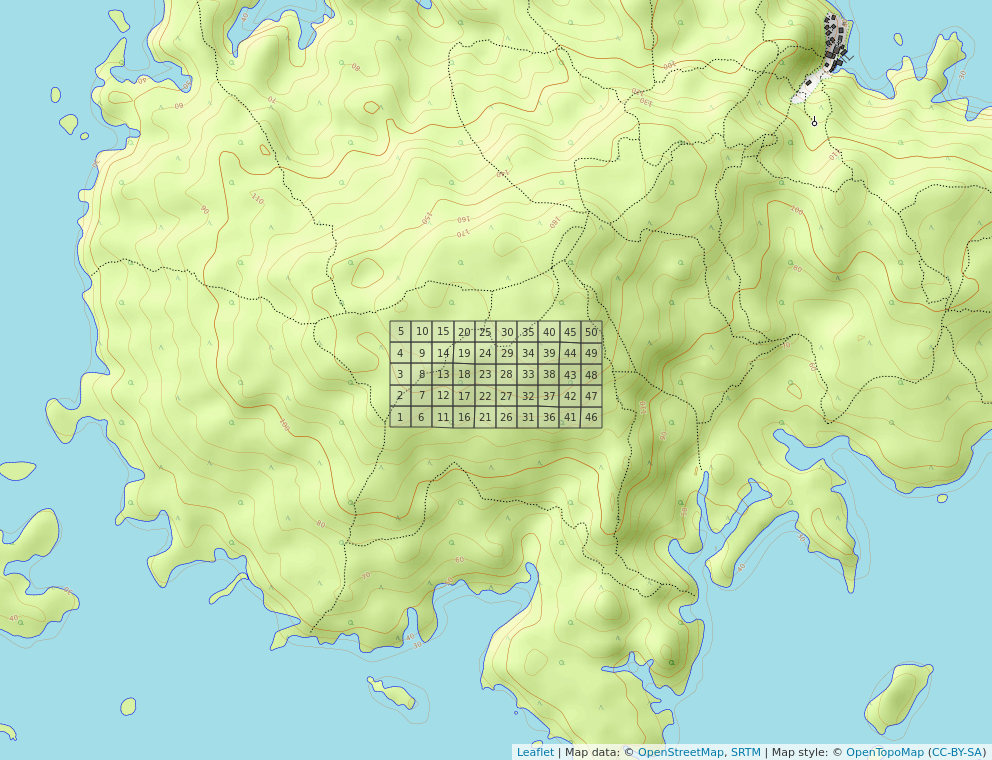
\includegraphics[width=1.00000\textwidth]{mapa_cuadros.png}
\caption{mapa de isla Barro Colorado cuadros\label{fig:bci_map}}
\end{figure}

Por igual empleo los cuadros de variables ambientales nominales y
numéricas de 1 hectárea de BCI, constituidas por categorías de edad,
habitat, geología y quebrada. Otros recursos de vital importancia son
las variables ambientales nominales de una hectárea de BCI, las
matrices, en especial de Spearman, de riqueza y abundancia de suelo, y
las de Hellinger de medición de asociación. La interacción con estas
fuentes de información ayudan a tener una aproximación más concreta
sobre la diversidad con relación a la familia tratada.

Los métodos que hasta el momento he señalado corresponden a los mapas en
los cuales aparece la parcela de 50 hectáreas en la isla Barro Colorado,
en donde se describen las variables ambientales ilustradas en matrices
que describen el comportamiento de dichas variables, y los patrones de
movilidad en el espacio que presentan las mismas, lo cual en lo adelante
permitirá comprender el mecanismo que siguen la fuerte asociación,
abundancia y riqueza de la familia en cuestión.

Todo lo anterior obedece a la parte de datos exploratorios, con
excepción de las matrices de Spearman y Hellinger que ya fueron
mencionadas y que corresponden a la sección de medición de asociación.
Está presente el segmento correpondiente a la medición de asociación, en
el que se presentan los modos Q y R, el primero referido a la medición
de asociación de sitios, en este caso por medio de la distancia, y la
similaridad de Jaccard. El modo R se refiere a la medición de la
asociación entre pares descriptores como son variables o especies,
también hago uso de la matriz de Hellinger. En el método de análisis
jerárquico, también se emplean los diagramas del árbol o dendrogramas
(método de cuerda y de Ward).

El análisis de agrupamiento, consiste en una agrupación sucesiva basada
en la repetición de un procedimiento dado de grupos de objetos, hasta
que estos encuentren su lugar, se basa en la construcción de
dendrogramas. El análsis jerárquico se caracteriza por tener un enfoque
aglomerativo, lo que implica un algoritmo ascendente, y la ordenación de
los subgrupos de objetos en un único grupo. Los algoritmos del análsis
jerárquico son los criterios de enlace, y estos a su vez se integran por
los siguientes tipos: Enlace simple, enlace completo y enlace promedio.
Los metodos de representación utilizados son: Agrupamiento aglomerativo
por enlace simple, agrupamiento aglomerativo por enlace completo, y
agrupamiento aglomerativo por enlace promedio.

También es notable la sección correspondiente a las técnicas de
ordenación y a las especies indicadoras.

La ordenación es una técnica de medición que busca determinar el grado
de asociación y de agrupamiento. Un objeto se caracteriza por sus
propiedades en un espacio n-dimensional donde cada dimensión es una
variable, un descriptor. A diferencia de la técnica de agrupamiento, o
como complemento de este, el análisis de ordenación abarca un conjunto
de técnicas que busca abarcar el tamaño ( dimensionalidad) de los datos.
El análisis de ordenación puede ser no restringido y restringido, en el
primer caso, las tendencias detectadas en el conjunto de datos suelen
estar no restringidas por otro conjunto. En el segundo caso las
tendencias detectadas en un conjunto suelen estar asociadas a otro
conjunto.

Se realiza el análisis de las especies indicadoras por medio del
estadístico de IndVal. Para el análisis de diversidad se emplean los
modos alpha y beta. Dentro de las técnicas de ordenación (restringida y
no restringida) las pruebas PCA, RDA, y CCA. Estas pruebas buscan medir
la similaridad entre los sitios con variables ambientales determinadas.
Y por último, para el análisis de ecología espacial se empleó el
correlograma con estadístico de Moran's I, que determina la existencia
de una correlación positiva o negativa.

En un correlograma, se aprecia un rectángulo cortado a la mitad de forma
horizontal, sobre este suelen alternarse barras verticales surcadas a la
mitad por un punto que representa el valor estimado (Moran's I) el cual
se lee asumiendo los valores por debajo o por encima de cero
(correlación negativa o positiva), que coincidan con dicho punto, estos
son los valores de la barra lateral izquierda. Estos puntos al franquer
la barra que representa los valores positivos y negtivos pues recrean la
autocorrelación positiva y negativa, que se expresa en sitios ubicados a
cierta cantidad de metros entre sí.

A menudo se define la biodiversidad como la variavilidad de organismos
presente en un lugar determinado, y muchos estudiosos han dejado su
impronta sobre este concepto a lo largo del tiempo. Por ejemplo, Harper
y Hawsworth, defienden que es el estudio de tres aspectos fundamentales:
Intraespecífica, interespecífica, y de ecosistemas, con los adjetivos de
genética, de organismos, y ecológica. Hubell ofrece una definición más
restringida y ajustada a la realidad actual: Biodiverisdad es sinónimo
de riqueza de especies y de abundancia relativa de especies en el
espacio en el tiempo. Magurran utiliza el término diversidad biológica y
biodiversidad como sinónimas y la define como la variedad y la
abundancia de especies en un estudio.

\section{Resultados}\label{resultados}

\subsection{Análisis Exploratorio de
Datos}\label{anuxe1lisis-exploratorio-de-datos}

A continuación muestro las mediciones de pH, mapa de pendientes, mapas
de abundancia, tanto global como de la familia, mapa de riqueza global y
de la familia, variables ambientales numéricas, y nominales en una
parcela de 50 hectáreas, integrada por subdivisiones de una hectárea,
todo ello correspondiente a la familia de las Moraceae. En el caso del
pH tenemos que es ácido, sgún los mapas y diagramas consultados, estas
condiciones para las Moraceae, y cualquier otra especie en condiciones
extremas, sería perjudicial. El pH del suelo es importante porque los
vegetales solo pueden absorver a los minerales disueltos y la variación
del pH modifica el grado de solubilidad de los minerales y nutrientes.
En el siguiente mapa, se pueden apreciar las medidas de pH presentes en
la isla de Barro Colorado en una parcela de 50 hectáreas, con un patrón
de distribución al oeste de la parcela en su variedad ácida (ver figura
\#\#2).

\begin{figure}
\centering
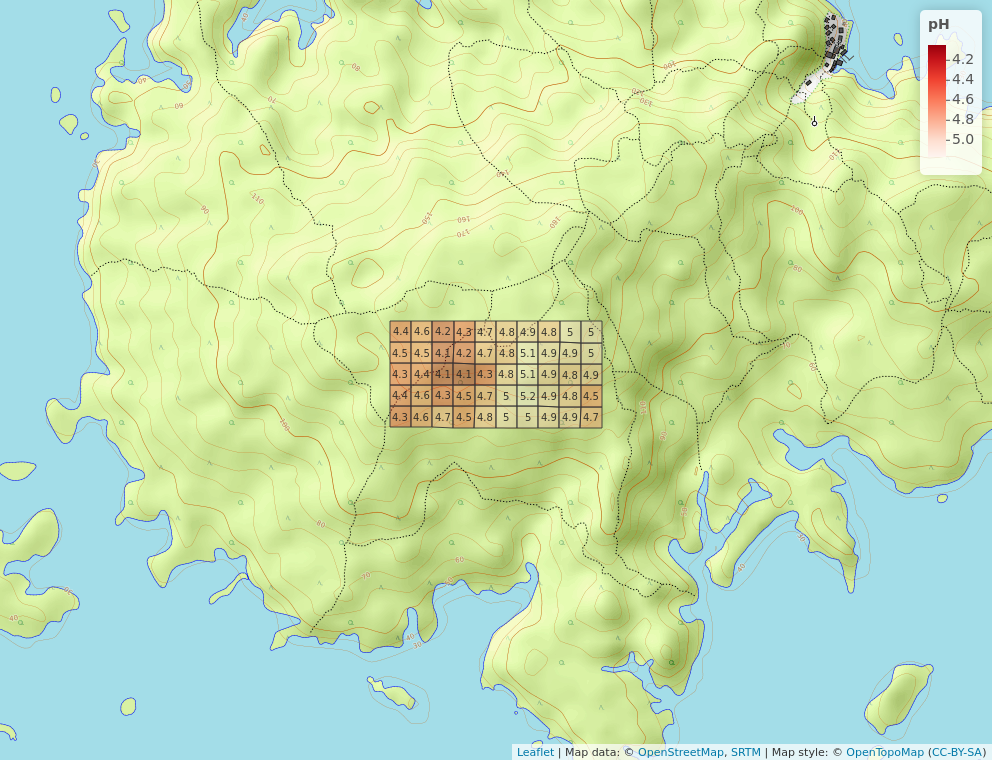
\includegraphics[width=1.00000\textwidth]{mapa_cuadros_ph.png}
\caption{mapa de la isla Barro Colorado cuadros ph\label{fig:bci_map}}
\end{figure}

Como se puede ver, el pH es eminentemente ácido, en una pacerla de 50
hectáreas, puesto que oscila en una escala de 0 a 6, con una
distribución que indica mayor concentración al oeste de dicha parcela.

En el mapa de abundacia global se advierten valores no lejanos de lo
ideal cuando se emplean parámetros de la muestra comprendidos entre 3600
y 5000, que en este caso sería una escala, en una parcela de 50
hectáreas. El Valor promedio que representaría cada hectárea en una
media hipotética sería de aproximadamente casi 4000 individuos de esta
familia, sin embargo tiende a cambiar cuando hablamos de riqueza. Si
bien existen dentro de esta familia, especies representativas de casi
todas las formas de vida leñosas, las formas más comunes entre las
especies de bibosi, son por un lado plantas hemiepífitas estranguladoras
o matapalos y por otro, plantas no epífitas con sistema propio de
sustento o higuerones (Fredericksen et al., n.d.,), (ver figura \#\#3).

\begin{figure}
\centering
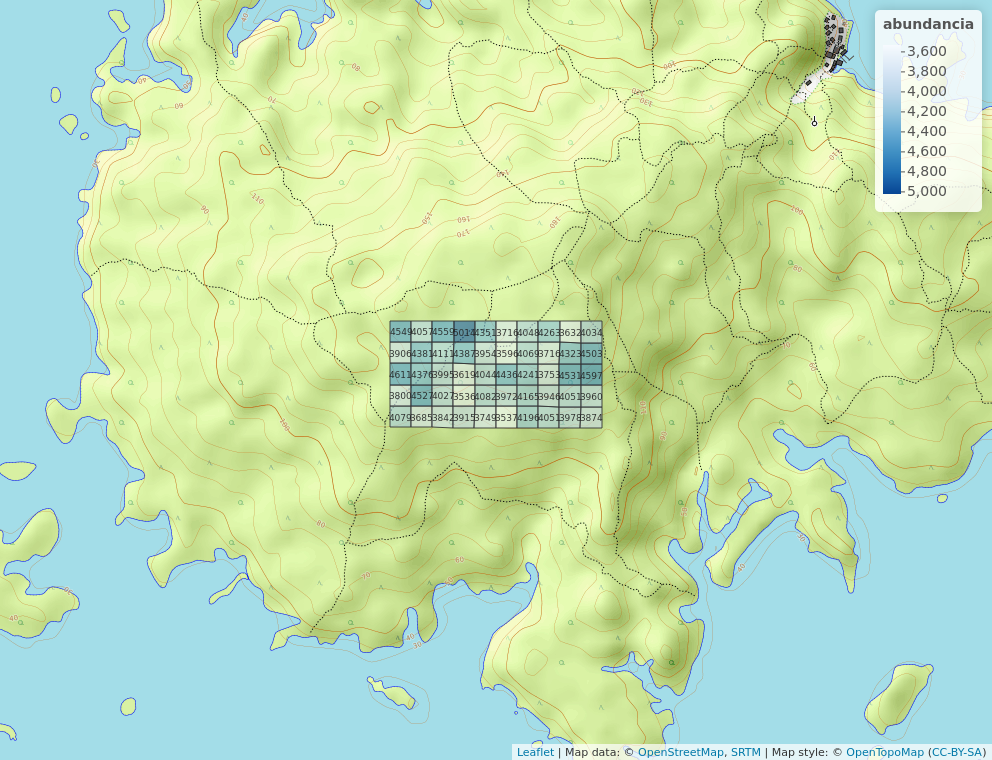
\includegraphics[width=1.00000\textwidth]{mapa_cuadros_abun_global.png}
\caption{mapa de la isla Barro Colorado abundancia global
\label{fig:bci_map}}
\end{figure}

En el mapa de abundancia de mi familia no se presenta tampoco que la
muestra por hectárea se aleja de forma marcada del parámetro empleado
para la parcela de 50 hectáreas, en este caso en un parámetro de entre
200 y 700 individuos, podría verificarse una especie de relación directa
entre el primer y segundo mapa.

En ambos casos cada hectárea adquiere valores próximos a la dimensión
numérica de individuos presentes en la parcela, para ello adjunto el
siguiente mapa sobre abundancia de mi familia (ver figura \#\#4).

\begin{figure}
\centering
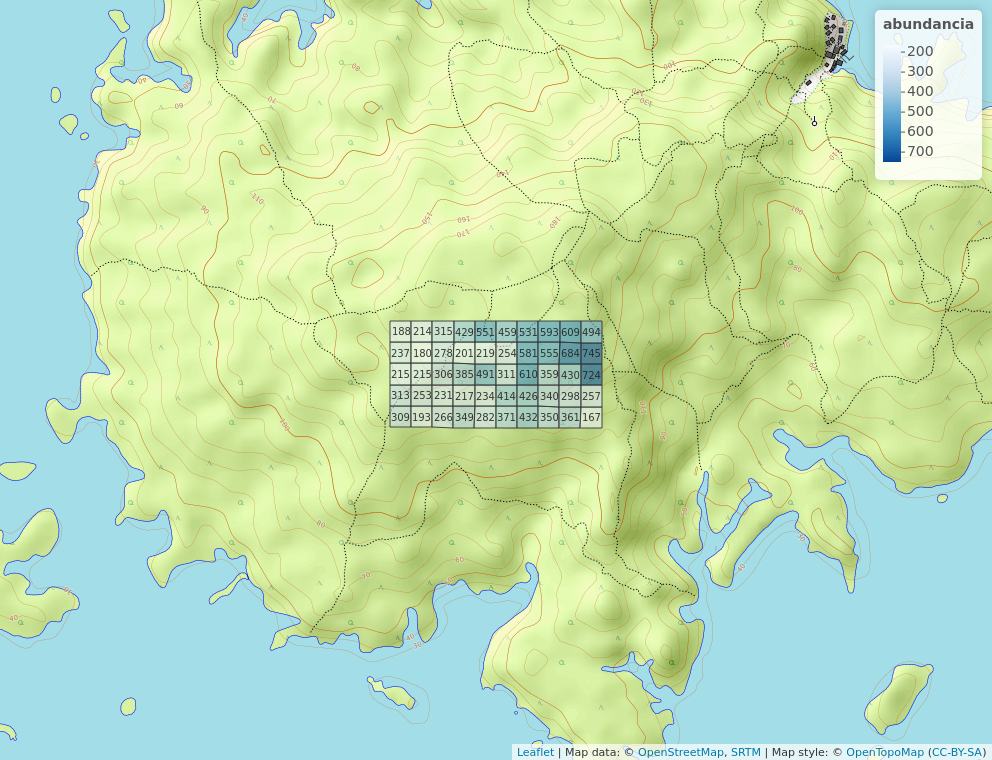
\includegraphics[width=1.00000\textwidth]{mapa_cuadros_abun_mi_familia.png}
\caption{mapa de la isla Barro Colorado abundancia de mi familia
\label{fig:bci_map}}
\end{figure}

Como puede comprobarse existen muchos individuos, en este caso citando
la abundancia, de una determinada especie de la familia de Moraceae en
una hectárea de la isla Barro Colorado, con un patrón de concentración
al noreste de la parcela, lo que muestra una amplia densidad para una
parcela de 50 hectáreas. Siendo estas plantas muchas veces ejemplares de
gran dimensión en muchos de los casos, se infiere que estas forman un
dosel impenetrable, típico de muchos bosques de la selva tropicla
centroamericana, en donde BCI no es la excepción. No solo estaríamos
hablando de Moraceae, sino de otras especies que forman la cubierta de
esta región intertropical.

La isla de Barro Colorado es realmente joven dentro de lo que es la
escala de tiempo geológico, solo tiene algo más de 100 años de
existencia lo que nos advierte de un relieve poco accidentado, debido en
gran parte a su tamaño, pero sobre todo a su edad.

En este sentido sería bueno apreciar las pendientes, y ver el valor de
la altitud en esta especie de enclave marítimo, lo que también favorece
la existencia abundante de ejemplares de Moraceae (ver figura \#\#5).

\begin{figure}
\centering
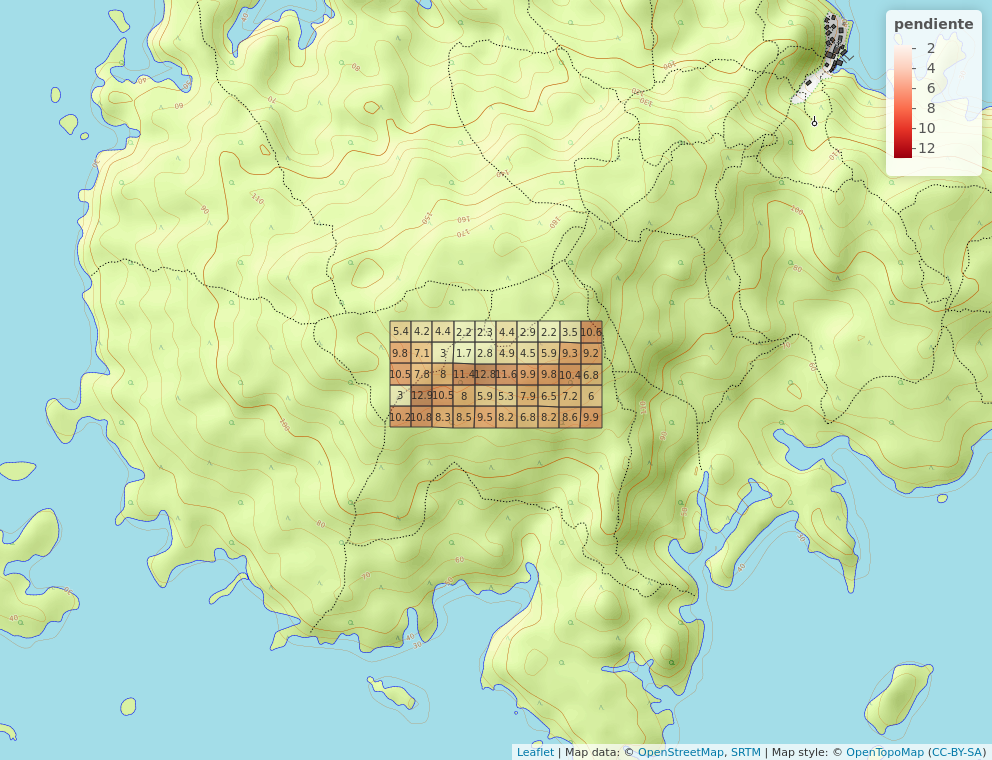
\includegraphics[width=1.00000\textwidth]{mapa_cuadros_pendiente.png}
\caption{mapa de la isla Barro Colorado cuadros y pendientes
\label{fig:bci_map}}
\end{figure}

Para una consideración general de la parcela de 50 hectáreas se destaca
gran pendiente, con un patrón de distribución al sur de la misma.

En el caso de las variables ambientales numéricas se obtiene los
siguientes valores (ver figura \#\#6)

\begin{figure}
\centering
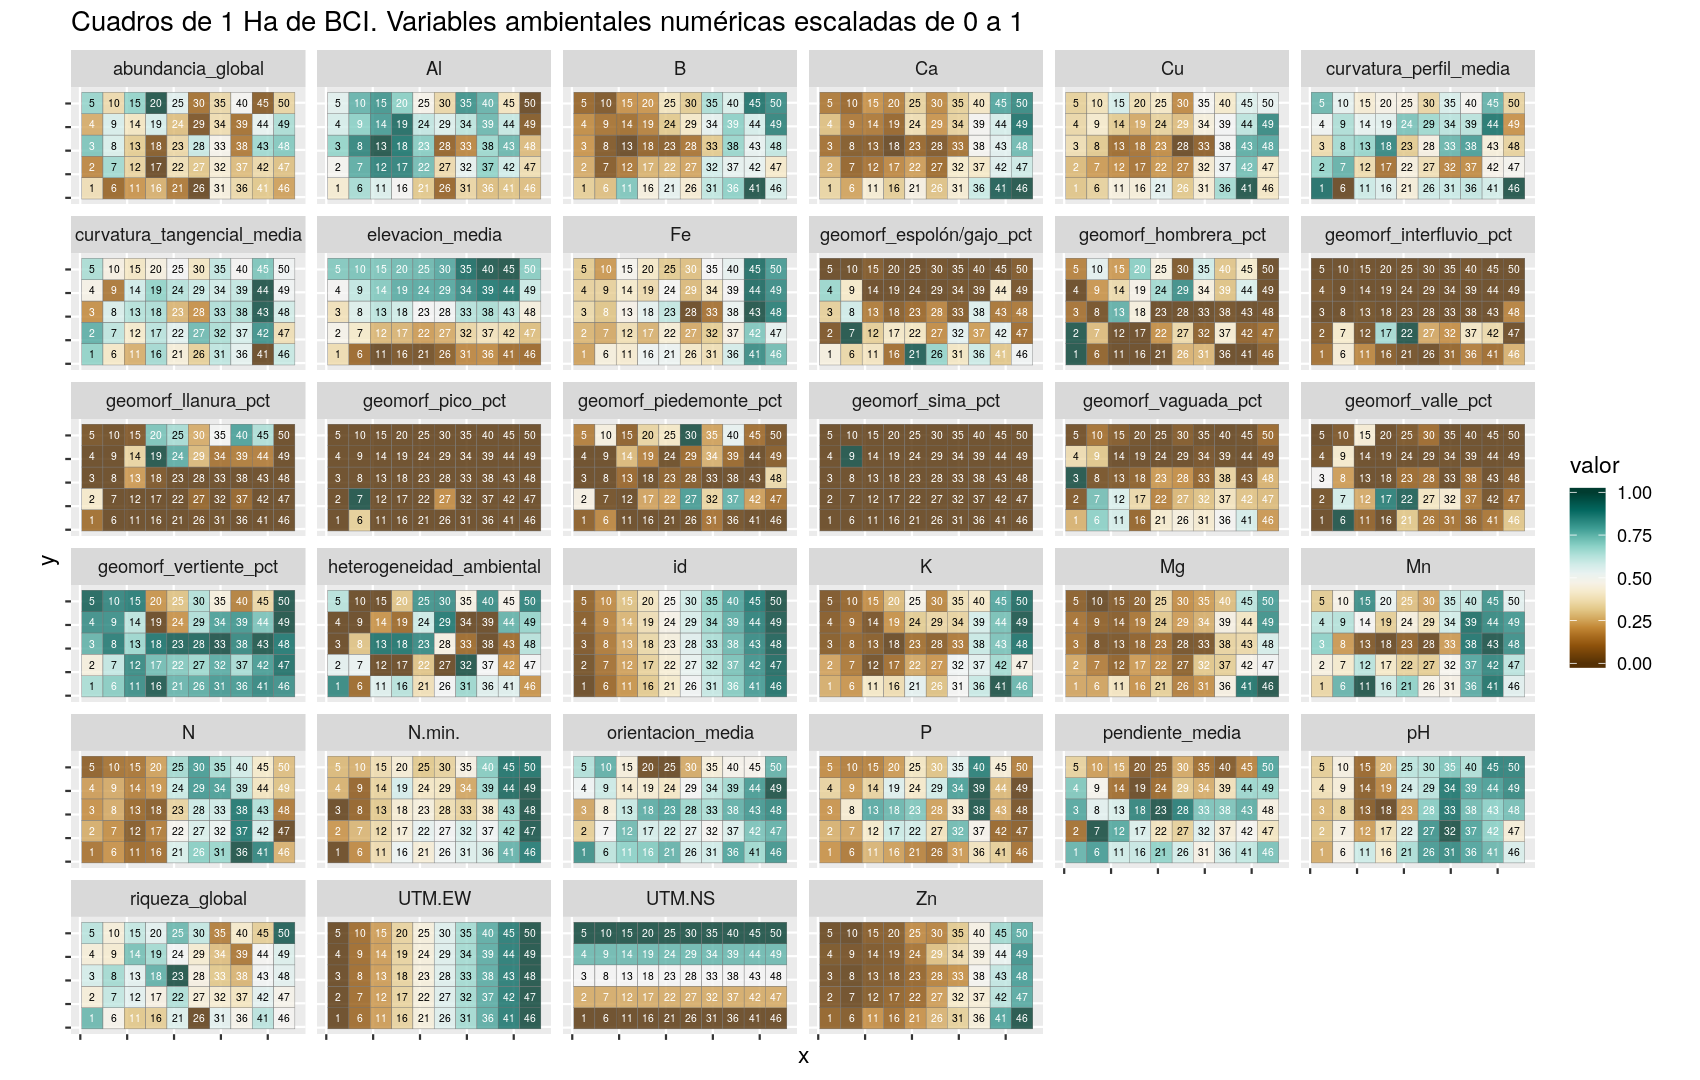
\includegraphics[width=1.00000\textwidth]{mapas_variables_ambientales_numericas.png}
\caption{mapa de la isla Barro Colorado variables ambientales numéricas
\label{fig:bci_map}}
\end{figure}

Aquí podemos ver una especie de síntesis de las informaciones que
ofrecen las variables ambientales de una hectárea, escaladas de 0 a 1.
En el caso de las geoformas, correspondientes a llanuras, se obtienen
valores grandes en un segmento de la escala que va de 0.00 a 0.25, lo
que refleja un terreno eminentemente llano. Con relación a las vrtientes
ocurre todo lo contrario, se obtienen valores grandes, en el segmento de
la escala que va de 0.75 a 1.00, lo que se refiere a mayor inclinación
en contraste con las tierras llanas. Otra geoforma como es el caso de
los valles, presenta valores muy pronunciados en los segmentos bajos de
la escala citada. Los valores de la escala muestran amplias diferencias
entre unas variables y otras, pero dentro de la misma escala, suele
verse la superioridad de una sobre otra.

En el mapa de variables ambientales nominales, se aprecia la dinámica de
algunas variables ambientales (ver figura \#\#7)

\begin{figure}
\centering
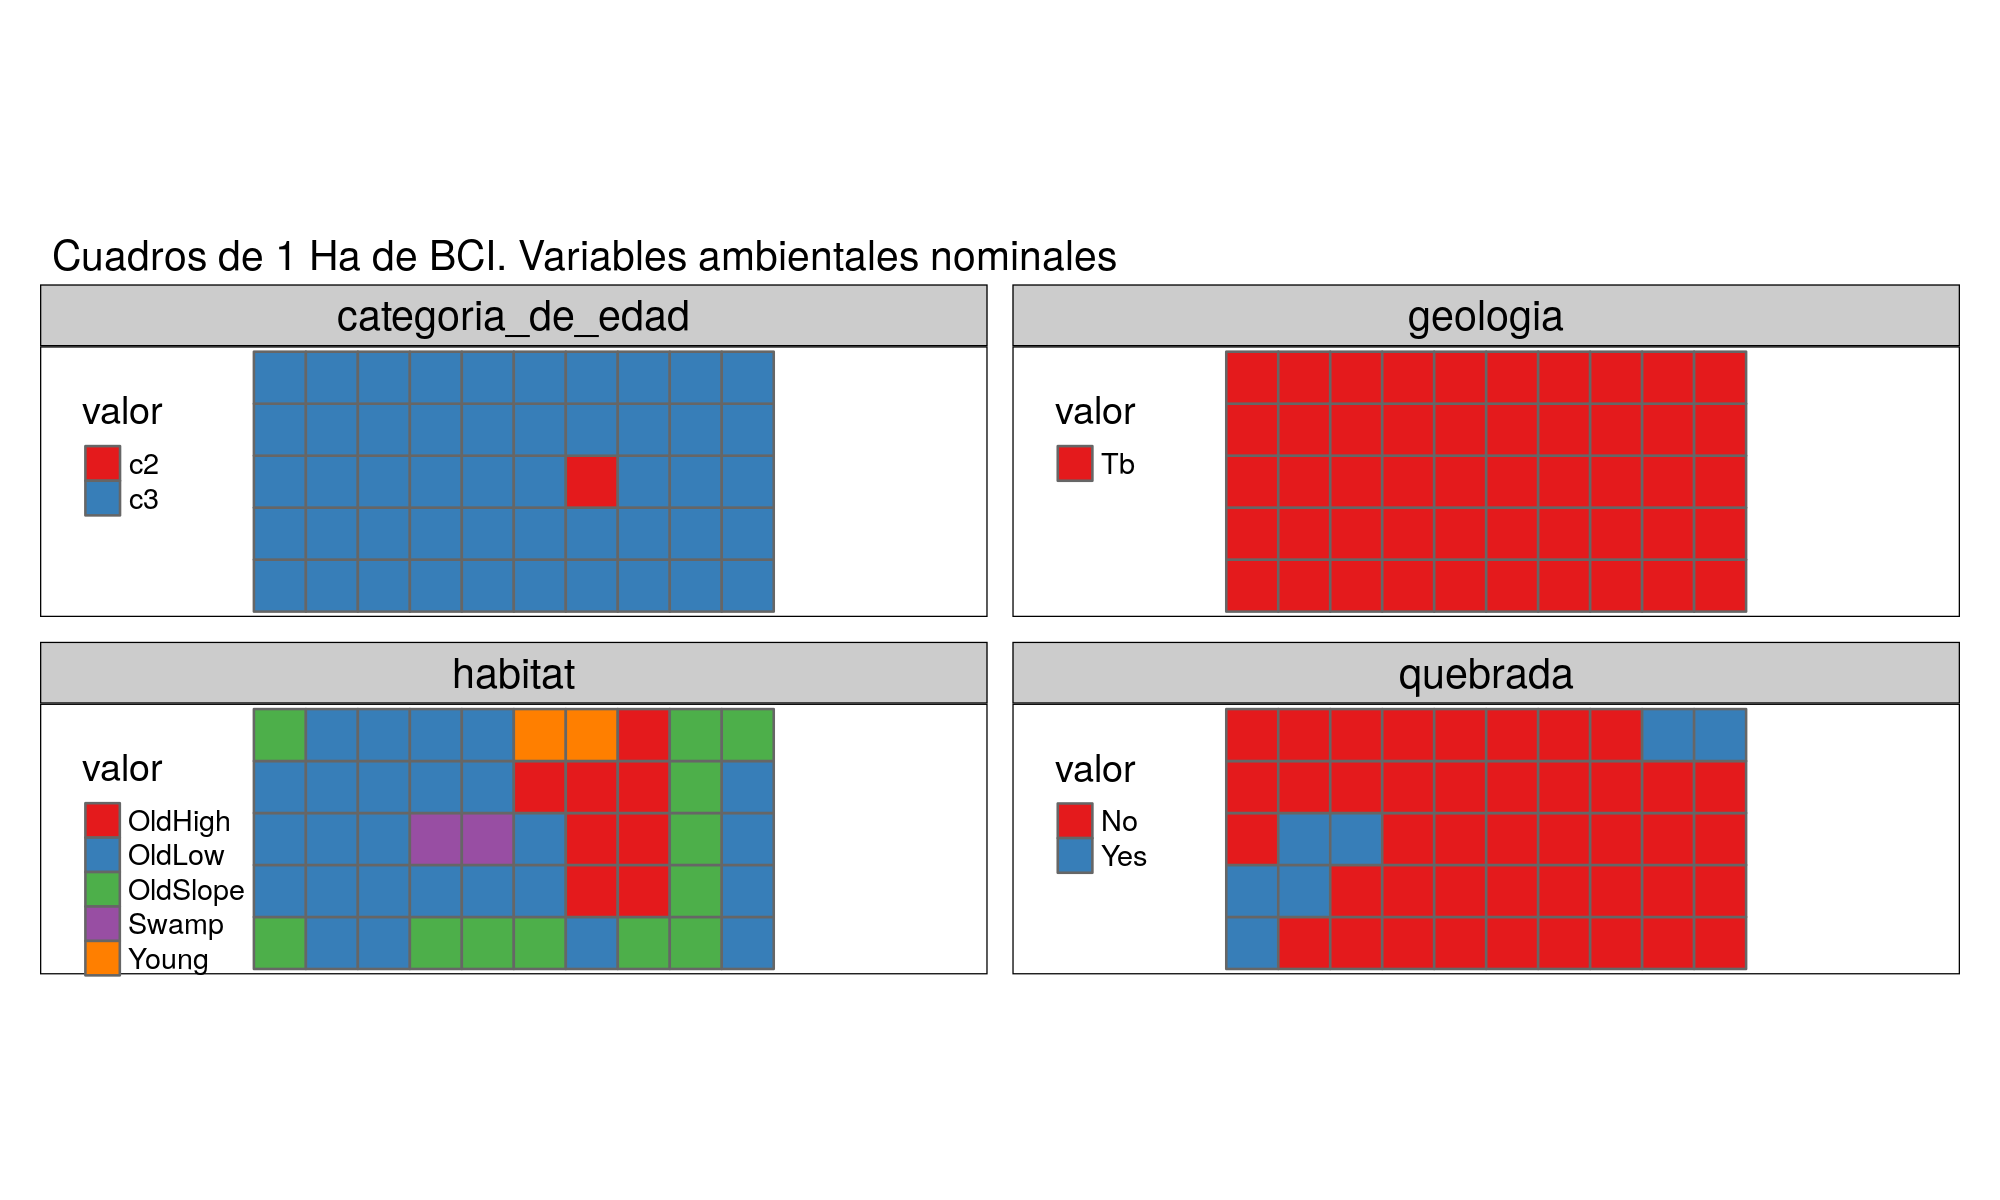
\includegraphics[width=1.00000\textwidth]{mapas_variables_ambientales_nominales_tmap.png}
\caption{mapa de la isla Barro Colorado variables ambientales nominales
\label{fig:bci_map}}
\end{figure}

En esta matriz se distinguen variables como la categoría de edad,
geología de la región, hábitat, y la quebrada. El hábitat de bosque
viejo en terreno alto (OldHigh), se destaca por su relativa minoría. En
tanto que el bosque viejo en relieve bajo (OldLow) es el más abundante.
El bosque viejo con pendiente (OldSlope), es relativamente abundante. El
pantano es escaso (Swamp), así también el bosque joven (Young). En
cuanto a la geología tenemos que el tipo de roca predominante es de tipo
intrusivo o plutónica. Las quebradas o barrancos son estrechos. Existen
dos grandes categorías dentro de la variable de edad, el bosque viejo en
terreno bajo, y el bosque viejo en terreno alto. De lo anterior se
infiere que existe más terreno bajo con bosque viejo en BCI en una base
gelógica joven, que con las demás variables.

El mapa de riqueza presenta un formato similar a los de abundancia, con
comportamientos diferenciados por hectárea, comparados con la parcela de
50 hectáreas. En el siguiente mapa puede apreciarse la riqueza de la
famiia botánica bajo estudio (Moraceae) por hectárea (ver figura \#\#8).

\begin{figure}
\centering
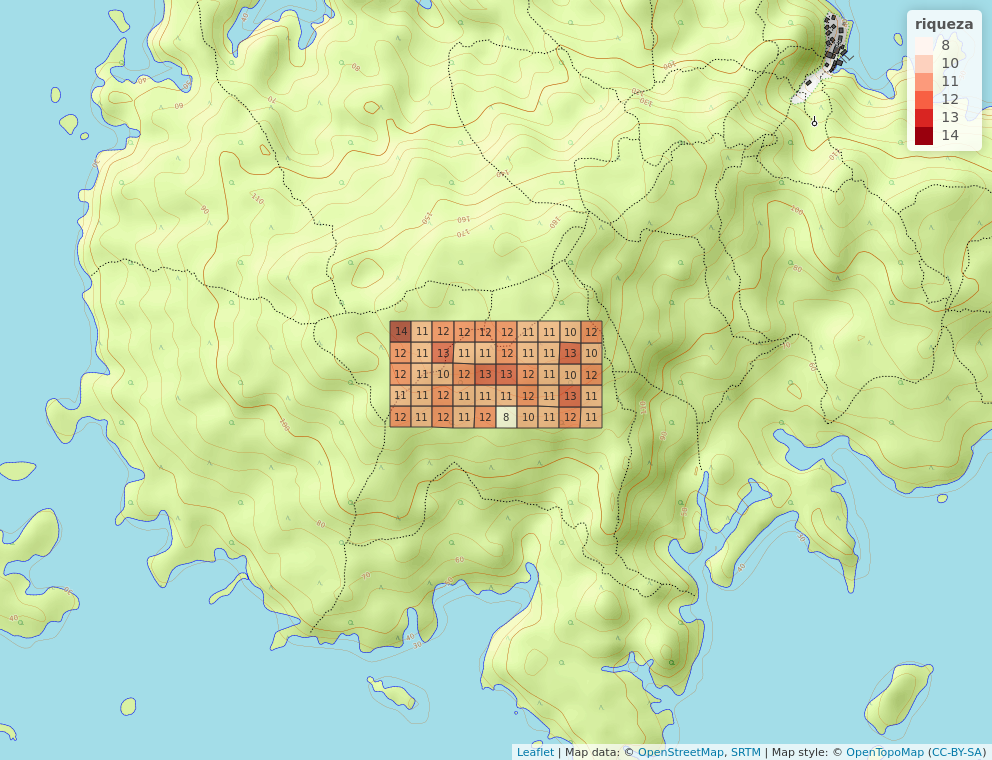
\includegraphics[width=1.00000\textwidth]{mapa_cuadros_riq_mi_familia.png}
\caption{mapa de la isla Barro Colorado cuadro de riqueza mi familia
\label{fig:bci_map}}
\end{figure}

En esta parte puede apreciarse que la riqueza es casi la misma por
hectárea, acercándose al nivel superior de la escala, así se puede
asumir que el grado de dispersión de algunos individuos de la familia
Moraceae es casi nulo. Existe una gran riqueza de estas plantas que
ayudan en gran parte a mantener este grandioso ecosistema.

Ya para el mapa de riqueza global se advierten mayores contrastes por
hectárea, pero igual se impone la diversidad, la multiplicidad de
individuos es asombrosa (ver figura \#\#9). La riqueza global presenta
un patrón de distribución noroeste-sureste.

\begin{figure}
\centering
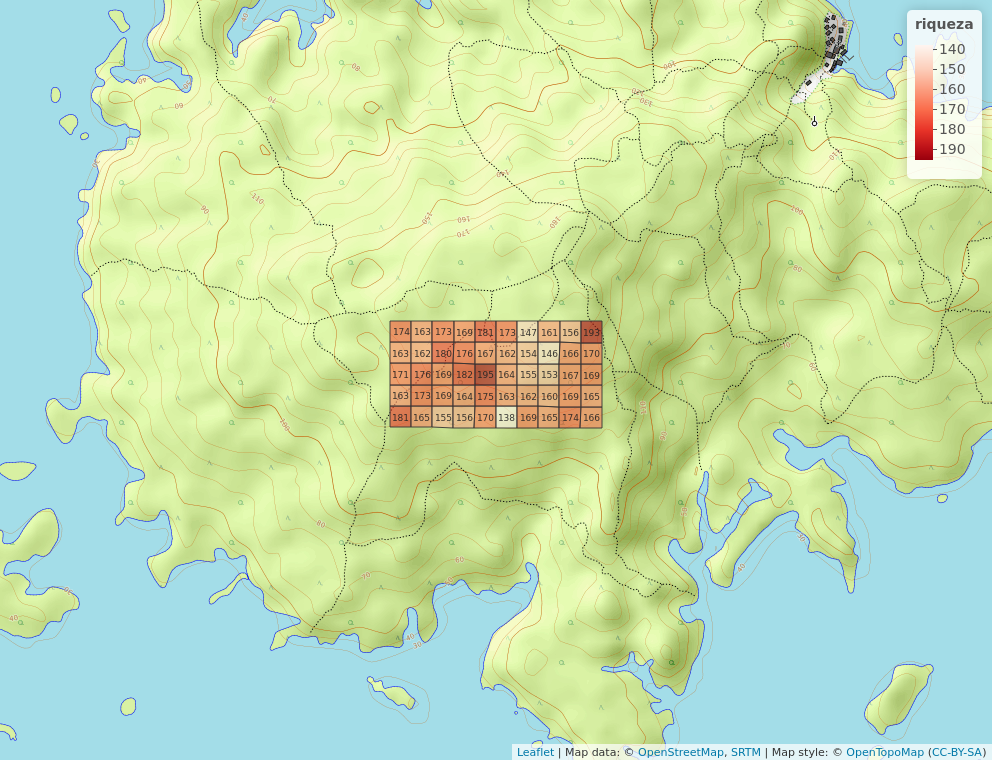
\includegraphics[width=1.00000\textwidth]{mapa_cuadros_riq_global.png}
\caption{mapa de la isla Barro Colorado riqueza global
\label{fig:bci_map}}
\end{figure}

En los cuadros de variables ambientales, se registran las diferencias
entre unas y otras, se distinguen tierras bajas de otras no muy altas.
Pero no solo se analizan los rasgos geomorfológicos, otras variables
ofrecen tambien allí su concurso. Aprecen valores de pH, riqueza global
por igual, abundancia global, entre otras variables.

\subsection{Medición de Asociación (Modos Q y
R)}\label{mediciuxf3n-de-asociaciuxf3n-modos-q-y-r}

En esta parte se aborda lo que es la medición de asociación, tomando en
cuenta lo que son los valores de disimilaridad o distancia, así como las
matríces de correlación. Dentro de los modelos de medición de asociación
existen los modos Q y R, en este caso de la distancia o disimilaridad,
tenemos el modo Q que describe la distancia entre objetos cuantitativos.
La paradoja de Orlóci plantea que la distancia euclidea es más pequeña
entre sitios que no comparten especies que entre sitios que sí las
comparten. A continuación se presenta una matríz de disimilaridad (ver
figura \#\#10).

\begin{figure}
\centering
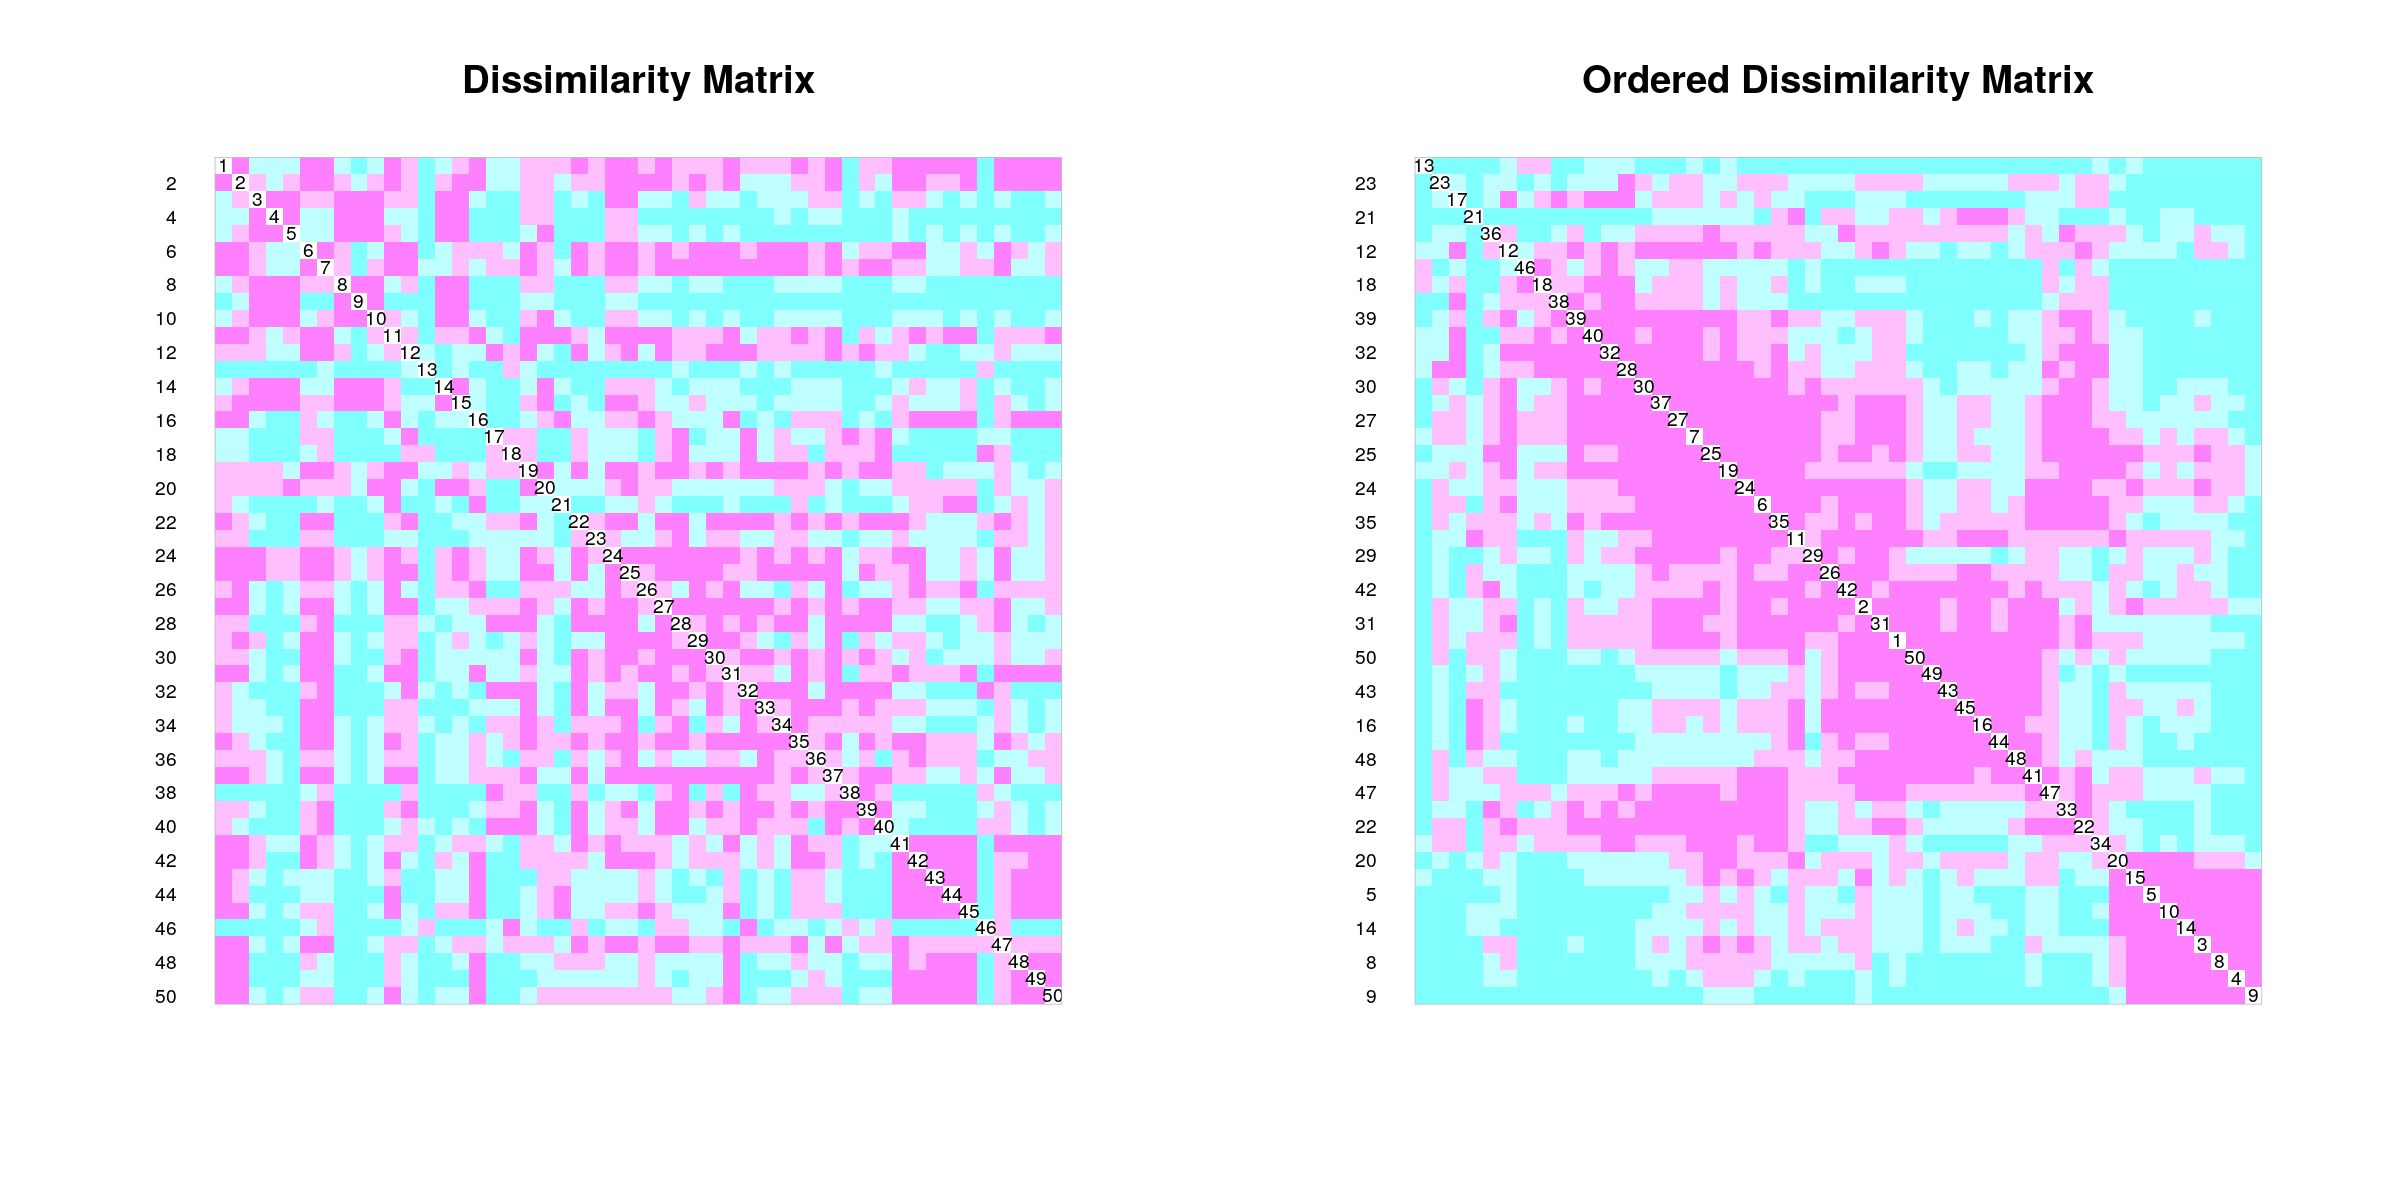
\includegraphics[width=1.00000\textwidth]{matriz_disimilaridad_hellinger.png}
\caption{mapa de la isla Barro Colorado matriz disimilaridad hellinger
\label{fig:bci_map}}
\end{figure}

La matrz de disimilaridad es una representación de la medición de
asociación entre objetos en el modo Q, como serían los sitios de
muestreo. En esta matriz se puede apreciar una fuerte asociación entre
objetos y esto lo indica la continuidad del color rosado (cuadro de la
derecha). En este caso nos referimos a la matriz de la derecha, que es
la matriz ordenada, a partir de la primera. Por ejemplo entre los sitios
40 y 35 existe una distancia muy pequeña entre sitios parecidos para la
matriz ordenada. La transformación Hellinger permite hacer la
interpretación en base a dos colores representativos: Color fucsia
(magneta, rosa) que equivale a corta distancia, muy similar, y el cian o
celeste que significa gran distancia o poco similar, todo esto con
relación a los elementos de la familia de las moraceae. Algunos de los
valores de disimilaridad o de distancia entre objetos que podemos
apreciar dentro de la transformación Hellinger son los siguientes: Entre
los sitios 2 y 1, tenemos que la distancia (dbl) es de 0.187, entre 3 y
1 es de 0.439, entre 4 y 1 es de 0.499, entre 5 y 1 es de 0.430, entre 6
y 1 de 0.297, entre 7 y 1 es de 0.280, entre 8 y 1 es de 0.492, entre 9
y 1 es de 0.584, entre 10 y 1 es de 0.425, y entre 11 y 1 es de 0.269 lo
que revela una escasa distancia o disimilaridad entre los objetos.

A continuación presento una versión mejorada de la matríz ordenada de
datos cuantitativos de especies (abundancia) con fuerte asociación en la
diagonal (ver figura \#\#11).

\begin{figure}
\centering
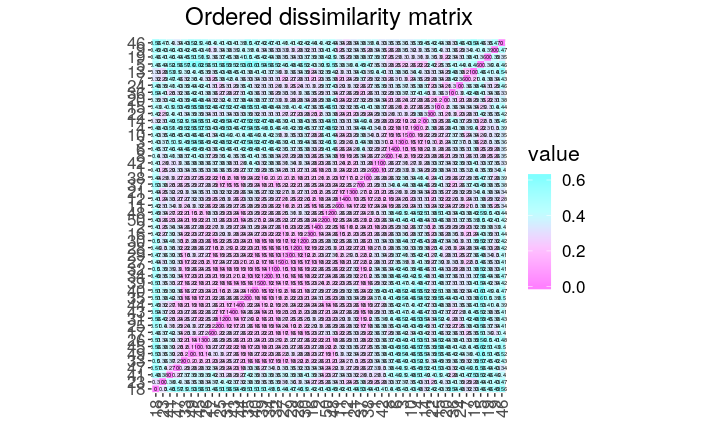
\includegraphics[width=1.00000\textwidth]{matrizdedisimilaridad.png}
\caption{mapa de la isla Barro Colorado matriz disimilaridad
\label{fig:bci_map}}
\end{figure}

En esta matriz de disimilaridad o de distancia vienen a recrearse los
anteriores casos de abundancia de los mapas de la Isla de Barro
Colorado. En la diagonal se pueden apreciar los sitios que poseen
características similares con la menor distancia(color rosado), mientras
que en los demás lugares se aprecian lugares con características
similares a mayor distancia y con una menor asociación (color cian o
celeste). Hasta el momento me he centrado en el modo Q que mide el nivel
de asociación por medio de la disimilaridad o similiridad. Algo
sumamente importante dentro del modo Q, en este caso basándome en datos
binarios (presencia/ausencia) es la famosa distancia de Jaccard, la
misma se puede expresar como la proporción de especies no compartidas.
Para el caso correspondinte de los datos de moraceae, la distancia (dbl)
muestra los siguientes resultados para algunos sitios: Entre 2 y 1, la
distancia es de 0.22, para 3 y 1 es de 0.33, entre 4 y 1 es de 0.222,
para 5 y 1 es de 0.3, para 6 y 1 es de 0.333, para 7 y 1 es de 0.222,
para 8 y 1 es de 0.333, para 9 y 1 es de 0.333, para 10 y 1 es de 0.4, y
para 11 y 1 es de 0.333, evidenciando en este caso una fuerte
asociación.

La similaridad es la proporción de objetos compartiods entre sitios, en
la siguiente gráfica de la matriz pueden apreciarse las espcecies
compartidas entre sitios (ver figura \#\#12).

\begin{figure}
\centering
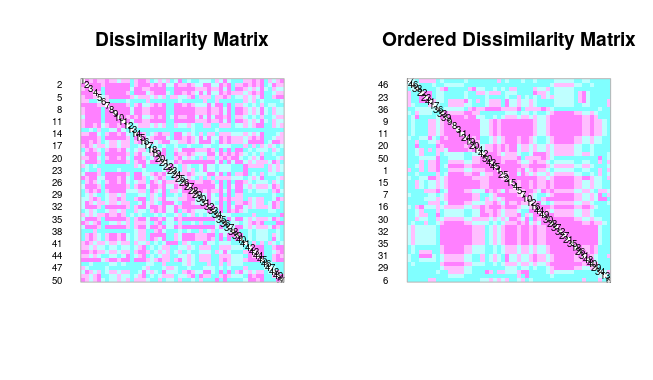
\includegraphics[width=1.00000\textwidth]{matriz_similaridad.png}
\caption{mapa de la isla Barro Colorado matriz disimilaridad
\label{fig:bci_map}}
\end{figure}

Pueden notarse en los bloques de colores las especies compartidas entre
sitios, y que son exclusivas de dichos sitios. Por ejemplo para las
variables a, b y c, que se desprenden de la fómula, incluida en los
scripts reproducibles que sirven de soporte a este trabajo, de la
similaridad, donde a representa el número de especies compartidas, b es
el número de especies exclusivas del sitio 2 y c el numero de especies
exclusivas del sitio 1. La cantidad de especies compartidas entre sitios
con relación a las moraceae es grande, esto debido a la ausencia de
ceros, hecho que en la paradoja de Orlóci refleja cercanía según la
distancia euclídea que hace ver próximos los lugares o sitios que no
comparten especies o individuos.

En el modo R se mide la asociación entre pares descriptores, es decir
variables o especies, mediante la covarianza y la correlación. Por
ejemplo para las variables a, b y c, que se desprenden de la fómula de
la similaridad, donde a representa el número de especies compartidas, b
es el número de especies exclusivas del sitio 2 y c el numero de
especies exclusivas del sitio 1.

Un ejemplo ilustrativo sería el mapa de calor (ver figura \#\#13)

\begin{figure}
\centering
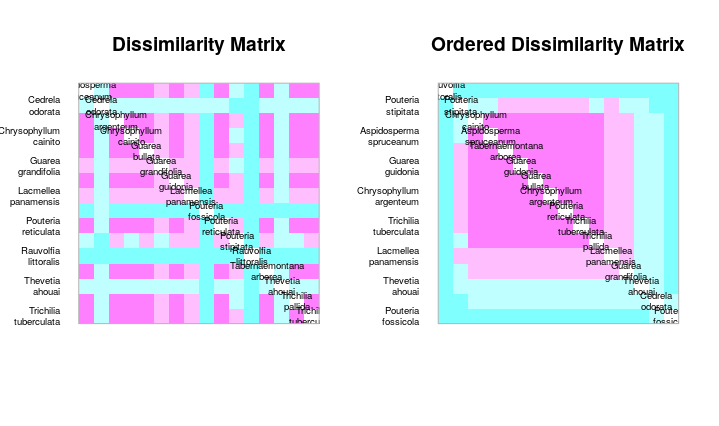
\includegraphics[width=1.00000\textwidth]{mapadecalor.png}
\caption{mapa de la isla Barro Colorado mapa de calor
\label{fig:bci_map}}
\end{figure}

En el mapa de calor mostrado se percibe una relación de dependencia en
la diagonal de la derecha, esto es lo que se mide en el modo R, la
asociación entre elementos descriptores, en este caso la abundancia de
especies como variables. Entre la \emph{Cainito aspidosperma} y la
\emph{trichinia tuberculata} se nota una fuerte dependencia, evidenciado
por la continuidad del color fucsia o rosa. Lo mismo no ocurre con los
colores de los bordes que reflejan franjas más pequeñas, y a su vez
degradadas, lo que evidencia ausencia de dependencia. Esto así cuando se
trata del modo R aplicado a datos cuantitativos de especies, que
reflejan la abundancia, al igual que el modo Q, el Modo R se aplica para
datos binarios, así tambien para la abundancia de variables
(coeficientes de spearman y pearson).

A continuación muestro una matriz de abundancia y riqueza de suelo según
el coeficiente de Spearman, con valores que aumentan y disminuyen de
este a oeste, y de norte a sur, los valores en rojo presentan los
valores más altos, y los azules los más bajos (ver figura \#\#14).

\begin{figure}
\centering
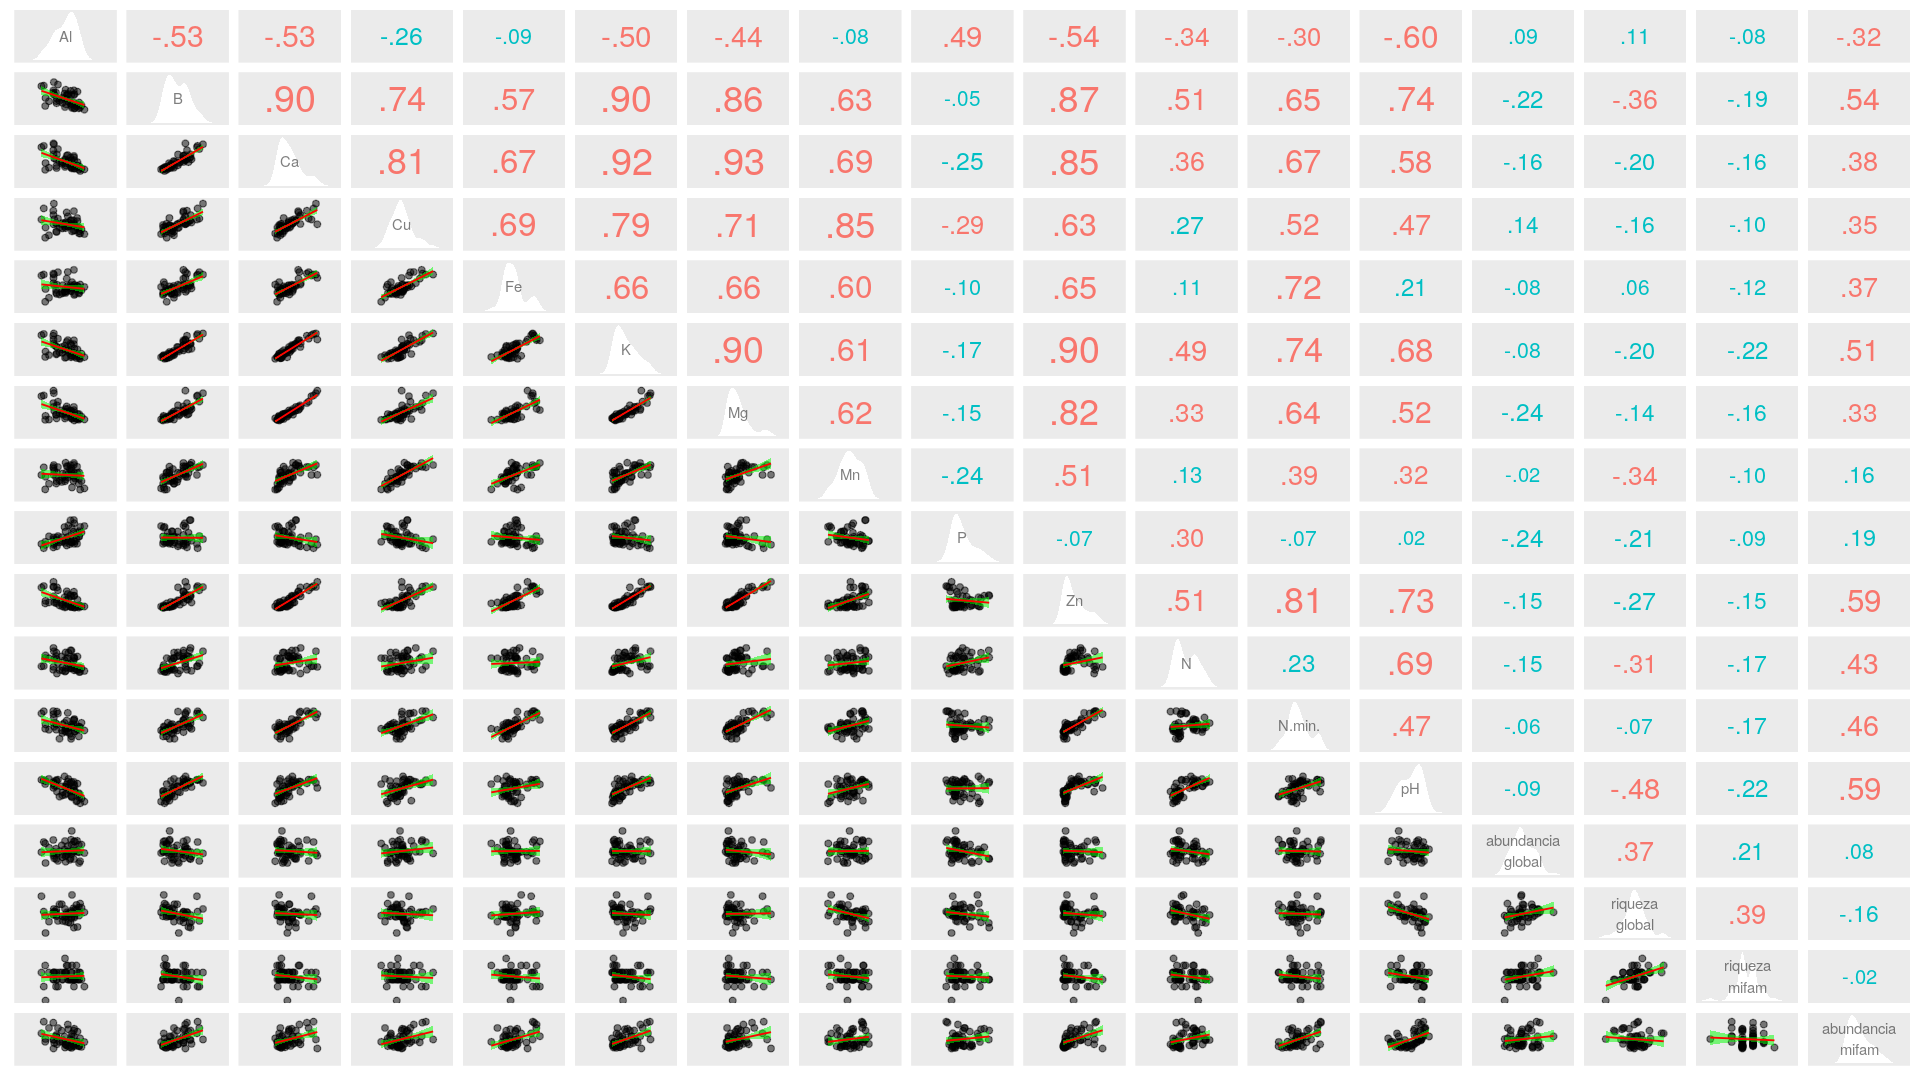
\includegraphics[width=1.00000\textwidth]{matriz_correlacion_suelo_abun_riq_spearman.png}
\caption{mapa de la isla Barro Colorado abundancia y riqueza de suelo
\label{fig:bci_map}}
\end{figure}

En la medición de asociación en los modos antes mencionados, se obtiene
una apreciación estadística de la distribución de sitios, especies y
variables ambientales presentes en la isla Barro Colorado que reflejan
la cuatificación de las comunidades de moraceas presentes en dicha isla,
así como la mayor o menor concentración de las mismas con relación al
grado de asociación presente en los sitios.

\subsection{Agrupamiento Jerárquico}\label{agrupamiento-jeruxe1rquico}

A continuación se muestran los resultados de esta sección
correspondiente a la familia de Moraceae.

\subsubsection{Agrupamiento Aglomerativo por Enlace
Simple}\label{agrupamiento-aglomerativo-por-enlace-simple}

\begin{figure}
\centering
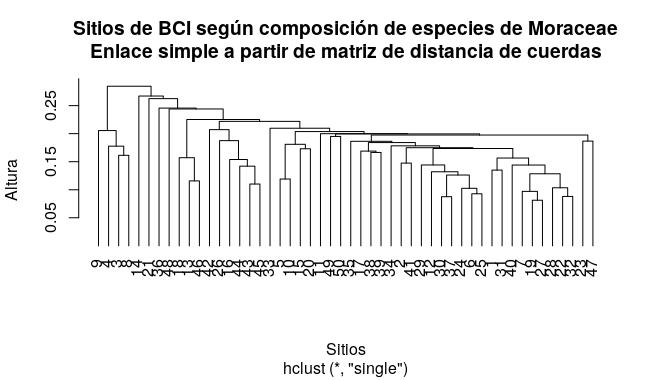
\includegraphics[width=1.00000\textwidth]{sitios_composicion_distancia_cuerdas.png}
\caption{mapa de la isla Barro Colorado sitios de composición por
distancia de cuerda \label{fig:bci_map}}
\end{figure}

Cuando se construye este dendrograma, empleando la menor distancia entre
sitios, se obtiene una matriz de cuerdas o matriz normalizada (ver
figura \#\#15). En este dendrograma se puede apreciar que en la parcela
de 50 hectáreas aún cuando se construyeran subgrupos cada vez más
pequeños para la familia de Moraceae, se formaría una innumerable
cantidad de los mismos, lo que pone sobre relieve la gran similaridad
entre sitios que albergan a especies de dicha familia, ya sea en función
de la abundancia o de la riqueza. Este dendrograma recuerda la forma de
una escalera (ver figura \#\#15).

\subsubsection{Agrupamiento Aglomerativo por Enlace
Completo}\label{agrupamiento-aglomerativo-por-enlace-completo}

\begin{figure}
\centering
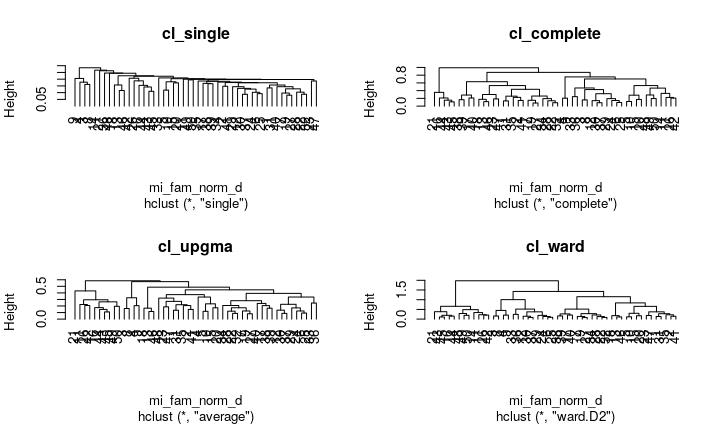
\includegraphics[width=1.00000\textwidth]{analisis_interpretacion_dendrogramas.png}
\caption{mapa de la isla Barro Colorado analisis interpretación
dendrogramas \label{fig:bci_map}}
\end{figure}

En esta imagen, aunque se ilustran los tipos considerados de
dendrogramas (ver figura \#\#16), nos interesa el completo. En el
agrupamiento aglomerativo por enlace completo, el criterio empleado es
la mayor distancia o menor similaridad, el vecino más lejano. En este
dendrograma se muestra una escalera pero con menor sucesión, se
distinguen grupos de dendrogramas como en el caso anterior, solo que en
esta ocasión los grupos con mayor distancia son poco numerosos en
contraste con los los grupos que presentan la menor distancia, y la
altura dominante para los cuadros mayores es de 0.8 en su generalidad.

\subsubsection{Agrupamiento Aglomerativo por Enlace
Promedio}\label{agrupamiento-aglomerativo-por-enlace-promedio}

\begin{figure}
\centering
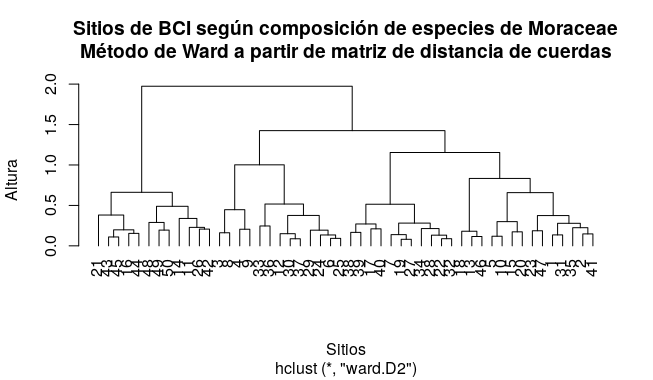
\includegraphics[width=1.00000\textwidth]{sitios_metodo_ward.png}
\caption{mapa de la isla Barro Colorado sitios de composición por
distancia de cuerda \label{fig:bci_map}}
\end{figure}

El método de Ward, aunque no es un método por enlace (ver figura
\#\#17), lo elijo por su fácil comprensión (en este caso sería el UPGMA,
para el caso de la media o promedio), recuerda la silueta de una
pirámide toscamente dibujada, con una interpretación visual más factible
que en los casos anteriores. Existe una regularidad en los subgrupos, lo
que refleja, al igual que en las secciones anteriores una fuerte
asociación, mayor similaridad que disimilaridad en las partes dominantes
o más visibles. Un ejemplo de visualización lo ofrece el modelo de
agrupación aglomerativa por enlace promedio, UPGMA, en el cual aparecen
siluetas aglomerativas y repetitivas que reflejan una continuidad en la
similaridad de los subgrupos.

\subsubsection{Interpretación de Agrupamiento
Jerárquico}\label{interpretaciuxf3n-de-agrupamiento-jeruxe1rquico}

En esta parte estamos a la altura de elegir métodos que nos permitan
minimizar la mayor cantidad posible de unidades de grupos en los
dendrogramas. Se establece la correlación cofenética y para la misma los
métodos convenientes son los de Ward y el UPGMA. En esencia consiste en
obtener la menor cantidad posible de siluetas que se distinguen por la
existencia de pequeños grupos de figuras. En la siguiente imagen pueden
apreciarse los cortes de las siluetas en tamaños menos complicados de
analizar y no muy distantes en su dimensión, por lo menos en los dos
primeros cuadros (ver figura \#\#18).

\begin{figure}
\centering
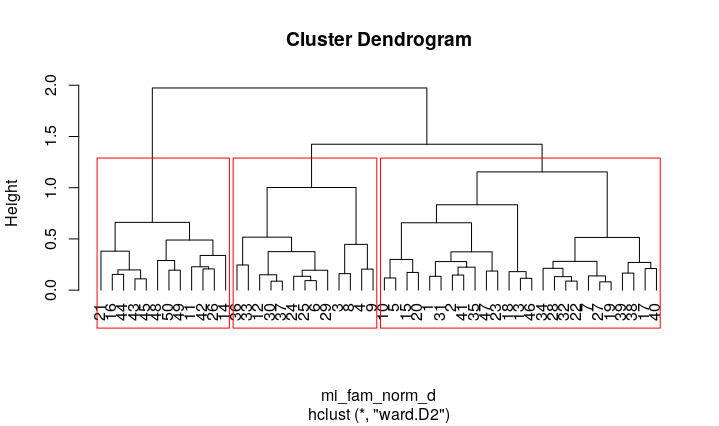
\includegraphics[width=1.00000\textwidth]{agrupamiento_dendrograma.png}
\caption{mapa de la isla Barro Colorado sitios de composición por
distancia de cuerda \label{fig:bci_map}}
\end{figure}

El método Ward es uno de los más ideales para elegir un dendrograma
único que permita apreciar por simple inspección el tamaño de las
siluetas, y el número de sitios que contienen, en este caso serían tres
cuadros de 12 y 13 sitios para el primer y segundo cuadro
respectivamente, y de 25 sitios para el tercero, todos a una altura de
1.3 aproximadamente dentro del dendrograma. En este dendrograma pueden
apreciarse las siluestas más fácilmente que en los ejemplos anteriores.

Una forma de ilustrar mejor la disimilaridad y la similaridad entre los
agrupamientos o dendrogramas es por medio del mapa de calor de la matriz
de comunidad fusionado con el dendrogrma. En eta ilustración se
distinguen los sitios que presentan mayor grado de asociación. Puede
verse que el dendrograma está cortado a la mitad, y los sitios que
presentan mayor similaridad o menor distancia están al centro y en los
extremos, por ejemplo, los grupos 13 y 18 presentan una fuerte
asociación, y en general los grupos dispuestos de forma vertical
presentan mayor similaridad que los dispuestos de forma horizontal (ver
figura \#\#19).

\begin{figure}
\centering
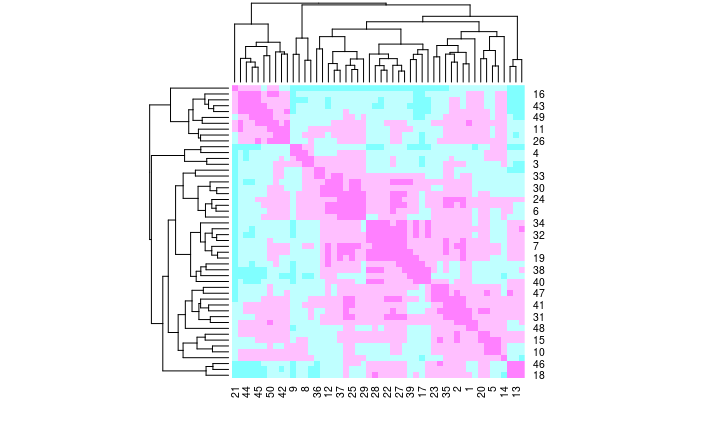
\includegraphics[width=1.00000\textwidth]{comparacion_dendrograma_mapa_calor.png}
\caption{mapa de la isla Barro Colorado sitios de composición por
distancia de cuerda \label{fig:bci_map}}
\end{figure}

\begin{figure}
\centering
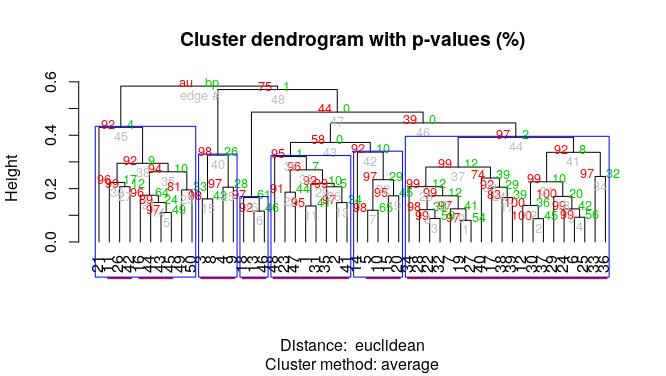
\includegraphics[width=1.00000\textwidth]{multiescalar_bootstrap.png}
\caption{mapa de la isla Barro Colorado remuestreo multiescalar por
Bootstrap \label{fig:bci_map}}
\end{figure}

En el mapa anterior pueden verse las probabilidades, y la anchura de las
siluetas de los cuadros que contienen los subgrupos con mayor
similaridad, lo que refleja los posibles cortes que se podrían hacer
sobre el dendrograma (ver figura \#\#20).

\begin{figure}
\centering
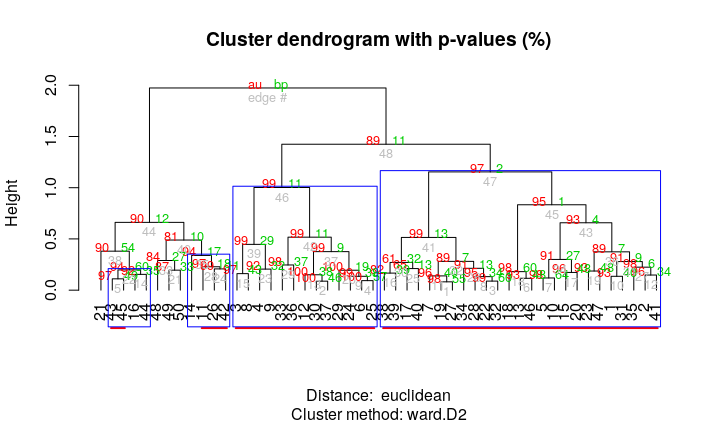
\includegraphics[width=1.00000\textwidth]{agrupamiento_dendrogramas_porcentajes.png}
\caption{mapa de la isla Barro Colorado dendrogramas y porcentajes
\label{fig:bci_map}}
\end{figure}

En el dendrograma anterior, también pueden notarse las probabilidades
por el método Ward (ver figura \#\#21)

Los dendrogramas, al igual que en los métodos de medición de asociación
permiten ver gráficmanete la dinámica de la distribución de las especies
de moraceae, sin embargo, estos nos ayudan a segmentar en grupos los
sitios con mayor cantidad de individuos o especies, dividiendolos en
cuadros a una mayor o menor altura, sería una forma de fraccionar en
grupos representativos lo que en principio parece desordenado y
monótono.

\subsection{Análisis de Variables Ambientales y
Mapas}\label{anuxe1lisis-de-variables-ambientales-y-mapas}

Dentro del análisis de agrupamiento, se haya incrustado el estudio de
las variales ambientales y los mapas. Desde un principio, en este
artículo, tanto la riqueza global como la de mi familia, han presentado
unos valores altos, y unos patrones de concentración y desplazamiento
por igual grandes.

Así se puede visualizar en el siguiente mapa (ver figura \#\#22)

\begin{figure}
\centering
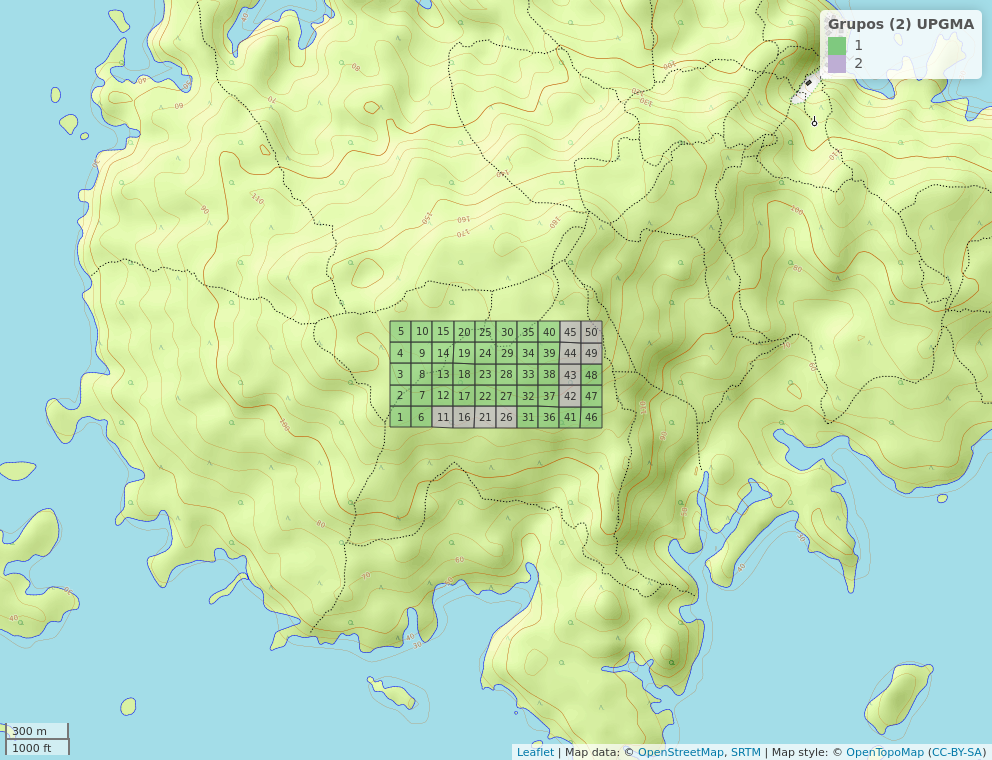
\includegraphics[width=1.00000\textwidth]{mapa_upgma_k2.png}
\caption{mapa de la isla Barro Colorado sitios de composición por
distancia de cuerda \label{fig:bci_map}}
\end{figure}

\begin{figure}
\centering
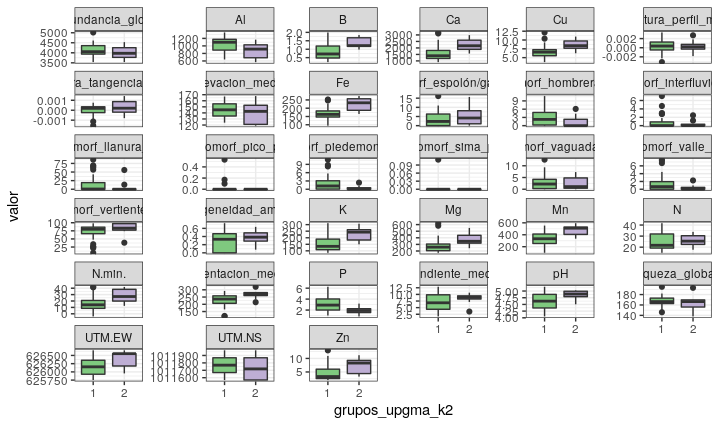
\includegraphics[width=1.00000\textwidth]{mapas_variables_ambientales.png}
\caption{mapa de la isla Barro Colorado mapa de variables ambientales
\label{fig:bci_map}}
\end{figure}

En el mapa adjunto, así como en el diagrama de cajas (ver figura
\#\#23), puede visualizarse el comportamiento de la mediana de las
variables ambientales, de la riqueza, así como también de abundancia. El
método UPGMA, presenta un patrón de distribución al este y al sur para
el grupo 2 de las variables ambientales dentro de la parcela de 50
hectáreas. Las varibles del grupo 1 de la parcela presentan un patrón en
todos los rumbos. Dentro de la riqueza, y la abundancia, los grupos 1 y
2, presentan valores no muy distantes, lo que evidencia el
condicionamieto ambietal de la isla, y que nuevamente refleja la fuerte
riqueza y asociación de las especies de Moraceae en dicho espacio
insular. Dentro de las variables ambientales de tipo geomorfológico, la
mediana para el grupo 1, naturalmente presenta mayores valores que
aquellos sitios de la misma parcela que se presentan en el grupo 2, pero
en cuanto a la concentración de elementos químicos en un número de
hectáreas más reducido (en este caso el grupo 2), representan mayor
valor para la mediana.

\begin{figure}
\centering
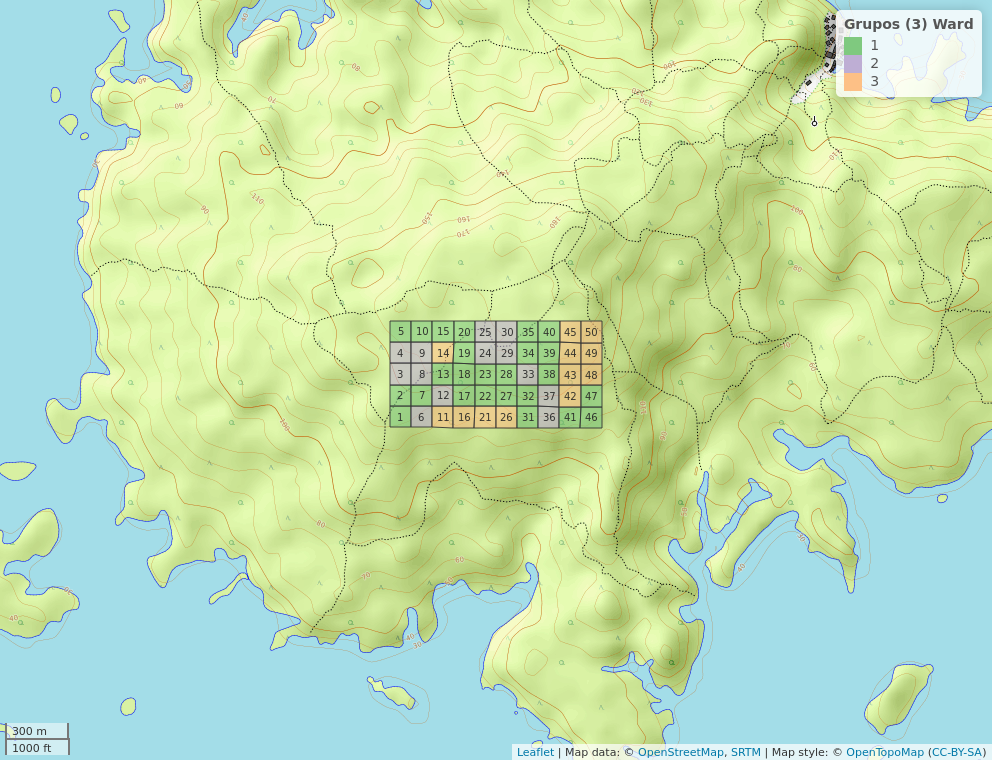
\includegraphics[width=1.00000\textwidth]{mapa_ward_k3.png}
\caption{mapa de la isla Barro Colorado grupos Ward k3
\label{fig:bci_map}}
\end{figure}

\begin{figure}
\centering
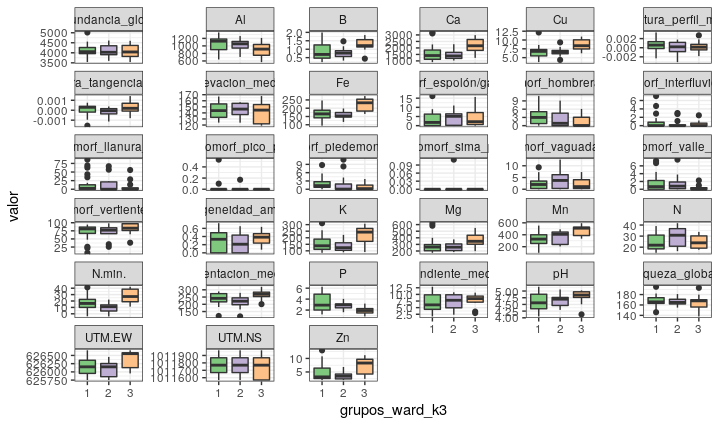
\includegraphics[width=1.00000\textwidth]{cuadro_cajas_ward.png}
\caption{mapa de la isla Barro Colorado cuadro de cajas Ward
\label{fig:bci_map}}
\end{figure}

Para el método Ward en el comportamiento de las varibles se presentan
tres sitios que muestran la dinámica de las variables ambientales dentro
de la parcela de 50 hectáreas con un patrón de distribución distinto al
caso anterior. Cuando relacionamos las varibles del diagrama de cajas
(ver figura \#\#25) que también se aprecian en el mapa (ver figura
\#\#24), puede corroborarse que estas se concentran más al centro de la
parcela, algunas al sur, y otras al este. Variables como el pH,
presentan altos valores de mediana en casi todas las hectáreas de la
parcela. También ocurre lo mismo con el nitrógeno. Para el caso de la
abundancia y la riqueza el valor de la mediana presenta valores
elevados, aunque en el caso de la primera las cajas o sitios ocupan
mayor espacio.

\subsection{Especies Indicadoras}\label{especies-indicadoras}

Para las especies indicadoras, tenemos que por especie indicadora se
entiende el grado de predicción que esta tenga dentro de un espacio bajo
estudio. Pueden darse casos de abunancia, y esos ejemplos de abundancia,
nos pueden llevar a la cocepción de grupos dentro de una familia. Dichos
grupos tienden a identificarse por el predominio de una variable
ambiental, ya sea un tipo de bosque, una concentración de pH, o de
ntrógeno. La aparición de estos grupos bajo el condicionamiento de
dichas variabes es lo que hace posible la existencia ordenada de los
mismos.

Existe el análisis de especies indicadoras por medio del método de
Inval, este método se aplica tanto para UPGMA, así como para Ward, se
verifica cuál es la especie que presenta el mayor indicador o
estadístico, la abundancia y la permutación. Para UPGMA, en el caso de
las Moraceae se registran dos grupos de una y cuatro especies
respectivamente. En el caso del primer grupo sería \emph{Perebea
xanthochyma} con una abundancia de 226, y un indicador (Inval) de 0.32,
tenemos en el segundo grupo: \emph{Pulsenia armata}, cuya abundancia es
de 993, y su indicador 0.774, \emph{Ficus tonduzzi} 23 y 0.459,
\emph{Tropis caucana} 136 y 0.454, y \emph{Tropis racemosa} con 218 y
0.420. En este primer grupo la especie indicadora es \emph{Perebea
xanthochyma} con los valores indicados y una permutación de 0.037, en el
segundo grupo: \emph{Pusenia armata} es la especie predictora de este
grupo por la abundancia que presenta, con un valor de permutación igual
0.001. El intervalo de confianza es pequeño, por ejemplo para
\emph{Brosimun alicastrum} va de -0.3597668 (-0.36) a 0.2896983 (0.29).

En el caso Ward, se registran por igual dos grupos, el grupo 3 y el
grupo 4 que resultaría de la suma del 2 y el 3 y que contiene una
especie indicadora. Sus valores de de abundancia e indicador estadístico
respectivamente son: \emph{Poulsenia armata} 993 y 0.785, \emph{Trophis
caucana} 136 y 0.538, \emph{Trophis racemosa} 228 y 0.435, y \emph{Ficus
tonduzii} 23 y 0.417.

Para el segundo grupo, tenemos la \emph{Maquira guianensis} con 1315 y
0.575. Para el tercer y cuarto grupo, las especies indicadoras son:
\emph{Pulsenia armata}, y para el cuarto grupo \emph{Maquiara guinensis}
con valores de permutación de 0.001 para ambos casos. Para el caso Ward
el intervalo de confianza es para la misma \emph{Brosimun alicastrum},
desde su límite inferior con -0.1289961 (-0.129) hasta su límite
superior de 0.41576092 (0.42).

\subsection{Análisis de Diversidad Alpha y
Beta}\label{anuxe1lisis-de-diversidad-alpha-y-beta}

En este artículo se emplean dos modalidades de estudio: Alpha y beta.

Para la diverisdad alpha sobre la familia en cuestión se muestran los
resultdos siguientes,

\begin{figure}
\centering
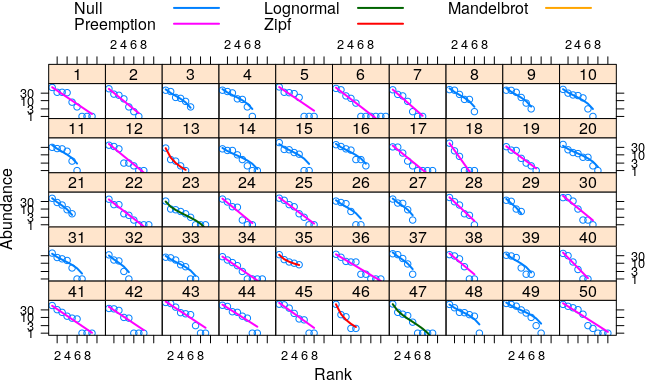
\includegraphics[width=1.00000\textwidth]{modelo_abundancia_especie.png}
\caption{mapa de la isla Barro Colorado modelo abundancia de especies
\label{fig:bci_map}}
\end{figure}

La gráfica anterior (ver figura \#\#26) representa la abundancia por
sitios, sitios de una hectárea, pero cada línea representa una métrica.
El gráfico también presenta cuáles sitios podrían mostrar mayor equidad.
Encontramos que las líneas de color verde y azul represental la mayor
abundancia de los lugares en los cuales se encuentran.

\begin{figure}
\centering
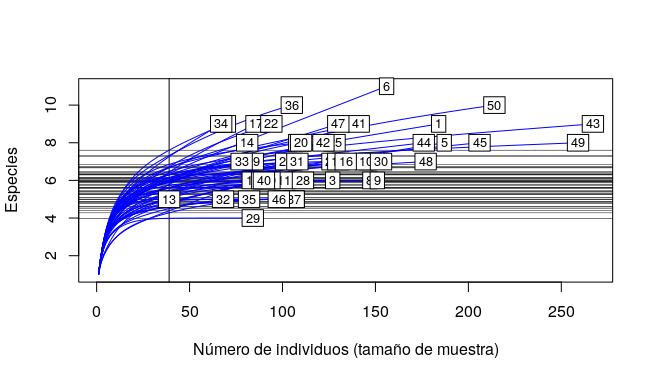
\includegraphics[width=1.00000\textwidth]{Numero_individuos.png}
\caption{mapa de la isla Barro Colorado número de individuos
\label{fig:bci_map}}
\end{figure}

En el digrama anterior (ver figura \#\#27) de curvas de rarefacción
puede apreciarse también el número de individuos por sitios. En este
diagrama puede apreciarse que prácticamente la totalidad de de sitios
poseen una cantidad de individuos superior a los 50 individuos, con
excepción del sitio 13 que posee unos 45 aproximadamente, y un escaso
número de sitios con una catidad superior a los 200 individuos. La mayor
cantidad de sitios comprende una riqueza en especies que va de los 50 a
los 200 individuos.

\subsection{Diversidad Beta}\label{diversidad-beta}

La diversidad beta se puede apreciar en segiente mapa de cuadros (ver
figura \#\#27), seguido de la gráfica (ver figura.

\begin{figure}
\centering
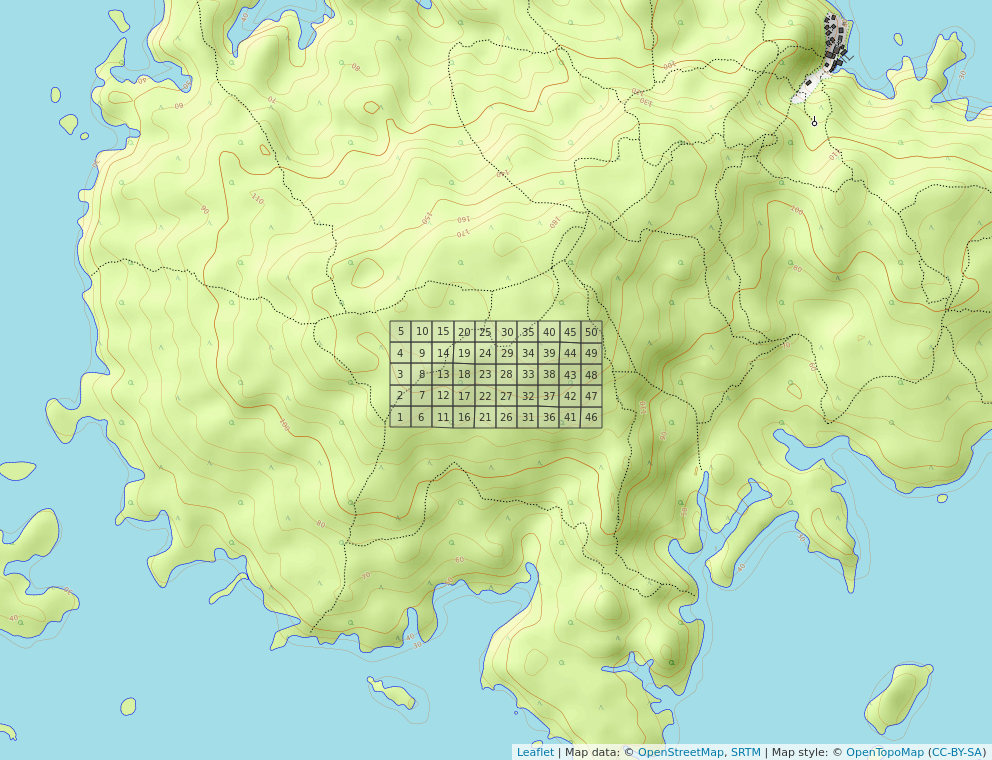
\includegraphics[width=1.00000\textwidth]{mapa_cuadros.png}
\caption{mapa de la isla Barro Colorado mapa cuadro diversidad beta
\label{fig:bci_map}}
\end{figure}

\begin{figure}
\centering
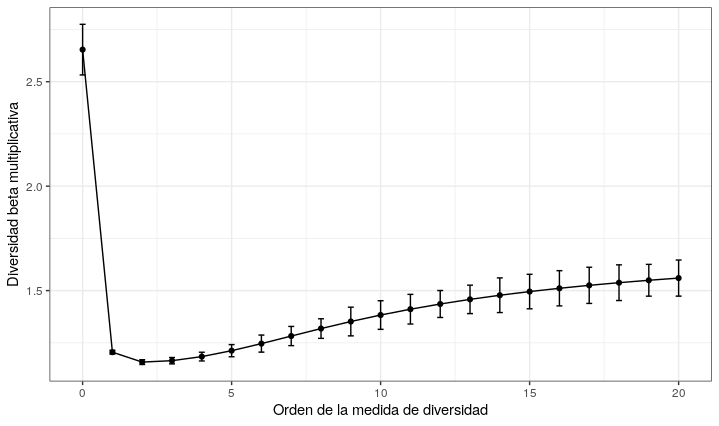
\includegraphics[width=1.00000\textwidth]{diversidad_beta.png}
\caption{mapa de la isla Barro Colorado mapa de calor
\label{fig:bci_map}}
\end{figure}

Para este tipo de diversidad, se presenta un patrón de distribución al
este de la parcela de 50 hectáreas y se aprecian las parcelas de una
hectárea que poseen la mayor cantidad de individuos por especies, al
oeste se aprecia una diversidad mucho más reducida. Este modo de
visualizar la variabilidad es más comprensible que en los casos
anteriores. En el gráfico (ver figura \#\#28) también puede apreciarse
mayor diversidad al este de la parcela.

\subsubsection{Análisis de Ordenación Simple (no restringida y
restringida)}\label{anuxe1lisis-de-ordenaciuxf3n-simple-no-restringida-y-restringida}

Las principales técnicas de análisis no restringido son: PCA (Análisis
de Componentes Principales), CA (Análisis de Correspondencia), PCoA
(Análisis de Coordenadas Principales), y NMDS (Escalamiento
multidimesional No Métrico).

Así se muestran para la familia de moraceae, empleando la técnica de
escalamiento PCA, la cual compara las componentes principales.

\begin{figure}
\centering
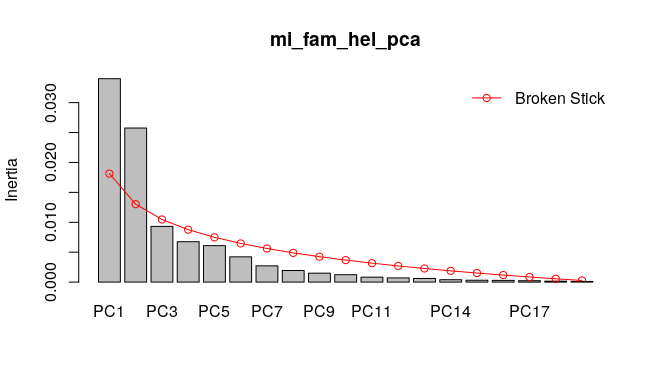
\includegraphics[width=1.00000\textwidth]{mi_fam_hel_pca.png}
\caption{mapa de la isla Barro Colorado diagrama de componentes
principales variables\label{fig:bci_map}}
\end{figure}

En este diagrama de componentes principales se puede visualizar un
decenso brusco de la medida de la inercia que pasa de 0.030 en la
componente principal 1 a 0.00 en la componente princioal 17 (ver figura
\#\#29).

\begin{figure}
\centering
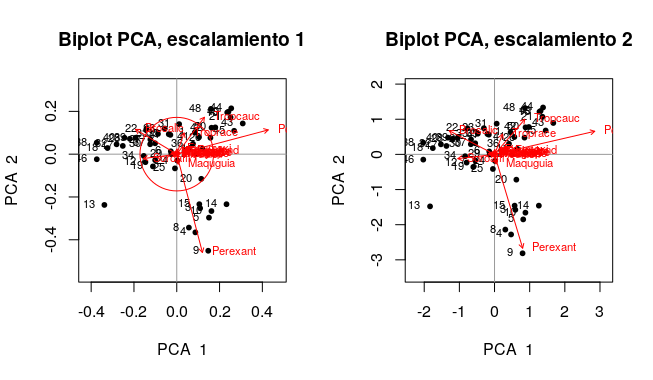
\includegraphics[width=1.00000\textwidth]{escalamiento_1_2.png}
\caption{mapa de la isla Barro Colorado diagrama de escalamiento 1 y 2
\label{fig:bci_map}}
\end{figure}

En esta técnica de escalamiento pueden visualizarse los grados de
asociación mediante un plano de coordenadas ortogonales. La cercanía que
describen los ángulos de las variables ambientales representa el grado
de asocición de las mismas. En el primer cuadrante (ver figura \#\#30)
predomina la distancia euclídea, en el segundo, la distancia de
Mahalanovich. Se forman nuves de puntos en los cuadrantes, estos puntos
representan los sitios, y como se puede ver en los gráficos, estos se
concentran más en el cuadrante negativo. Para ambos casos hay mayor
asociación al norte del plano.

\begin{figure}
\centering
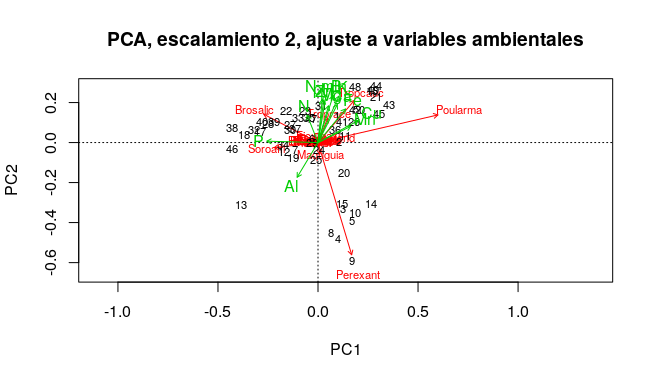
\includegraphics[width=1.00000\textwidth]{escalamiento_ajuste_2.png}
\caption{mapa de la isla Barro Colorado diagrama asociación de
variables\label{fig:bci_map}}
\end{figure}

En este diagrama (ver figura \#\#31) puede percibirse la fuerte
asociación que existe en las variables ambientales (color verde), por la
cercanía de los ángulos en la parte superior del plano. Hay mayor
asociación en la componente principal 2 que en la componente principal
1.

\subsubsection{Ordenación Simple
Restringida:}\label{ordenaciuxf3n-simple-restringida}

Para la ordenación restringida, las tendencias asociadas a un grupo de
ordenación se asocian a otro grupo. Las principales técnicas de
ordenación restringida son: Análisis de redundancia (RDA), Análisis de
redundancia basado en la distancia (db-RDA), Análisis de Correspondencia
Canónica (CCA), Análisis Discriminante Lineal (LDA), Curvas de
respuestas Principales (PRC), Análisis de Correspondencia conjunto
(CoCA, Análisis de Correlación Canónica (CCorA) y Análisi de Inercia
Conjunto (ColA).

En esta parte se mostrarán los resultados para RDA Y CCA. RDA combina la
regresión y elanálisis de componentes principales.

\begin{figure}
\centering
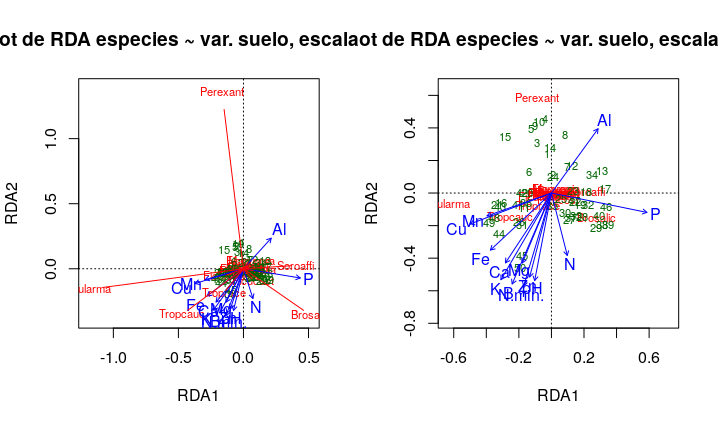
\includegraphics[width=1.00000\textwidth]{rda_escala_especies.png}
\caption{mapa de la isla Barro Colorado RDA diagrama de especies
variables\label{fig:bci_map}}
\end{figure}

\begin{figure}
\centering
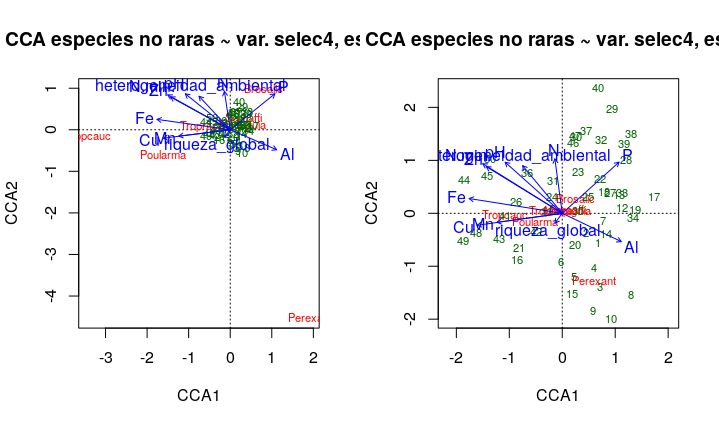
\includegraphics[width=1.00000\textwidth]{rda_escalamiento_escala_5.png}
\caption{mapa de la isla Barro Colorado RDA especies no raras
variables\label{fig:bci_map}}
\end{figure}

\begin{figure}
\centering
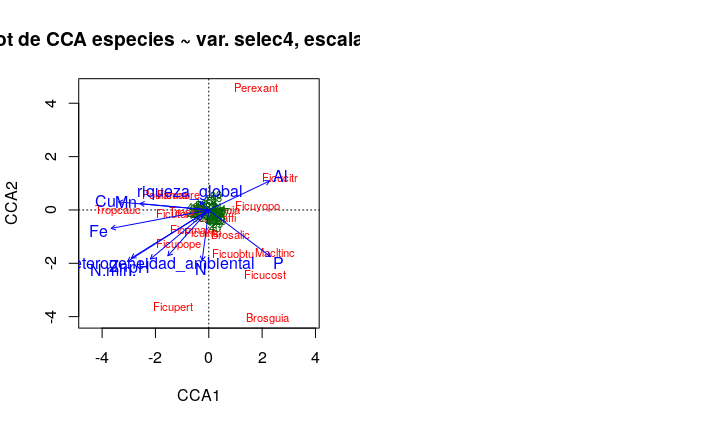
\includegraphics[width=1.00000\textwidth]{rda_especies_escala_4.png}
\caption{mapa de la isla Barro Colorado RDA digrama de especies
variables\label{fig:bci_map}}
\end{figure}

En estos planos bidimensionales puede apreciars el comportamiento de las
variables ambientales incluyendo el recurso suelo, de las especies, y de
especies no raras. en el primer diagrama (RDA) (ver figura \#\#32) puede
verse la fuerte asociación de los elementos químicos que integran el
suelo, descrita por las líneas azules que represental los ángulos en el
tercer cuadrante del plano. En el digrama de especies no raras (CCA)
(ver figura \#\#33) se percibe una fuerte concentración de sitios en el
tercer cuadrante, y es precisamente allí donde existe una menor
asociación entre elementos químicos (variables ambientales). Por ejemplo
el fósforo está presente en la mayor cantidad de sitios, y es un
elemento que se encuentra a una distancia angular considerada con
relación a los demás, lo mismo pasa con el alunminio. Para el cobre, el
manganeso y el hierro ocurre todo lo contrario.

En el último diagrama (ver figura \#\#34) correspondiente a CCA, existe
mayor asociación entre las especies en las zonas con predominio de
fósforo y aluminio, correspondiete a los cuadrantes 1 y 2 del plano.

\subsection{Análisis Espacial de Datos Ecológicos
(Autocorrelación)}\label{anuxe1lisis-espacial-de-datos-ecoluxf3gicos-autocorrelaciuxf3n}

Esta es una froma de observar los valores de las variables Ambientales
desde una perspectiva espacial, por medio de segmentos verticales,
parecidos a bastones, encerrados en cajas, se pueden ver de una forma
más comprensiva la dinámica del valor de correlación de las especies de
Moraceae que se vienen tratando, y que se pueden apreciar en el gráfico
o correlograma (ver figura \#\#35).

\begin{figure}
\centering
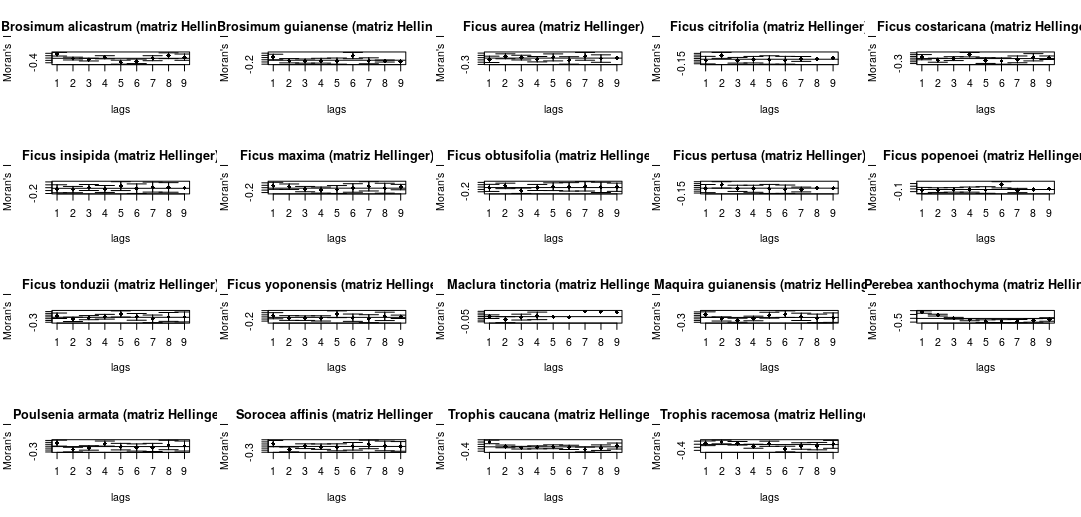
\includegraphics[width=1.00000\textwidth]{multiples_especies.png}
\caption{mapa de la isla Barro Colorado RDA digrama de especies
variables\label{fig:bci_map}}
\end{figure}

A partir de esta pequeña descripción del correlograma se puede entender
la dinámica espacial de algunas especies de Mooraceae. Como puede verse
existe una correlación más positiva que negativa entre las distintas
especies de moraceae. Lo que nuevamente viene a recrear la gran riqueza
predominante en las distintas especies de Moraceae, la similaridad qe se
hace visible en cada modo de estudio empleado.

\section{Discusión}\label{discusiuxf3n}

La abundancia y riqueza de la familia Moraceae, dentro de la isla Barro
Colorado, es vieja y asentada en terreno bajo, en su generalidad, con
una adaptación bastante ajustada a las condiciones de los factores
físico químicos de dicha isla, por lo general son plantas perennes, de
gran porte que sirven de alimentación a los individuos frugívoros que
allí habitan, constituyendo con su dosel el típico paisaje de la selva
tropical crentroamericana.

Como se pudo ver en los mapas, y los cuadros de variables, se presenta
gran riqueza y abundancia en espacios muy reducidos. Todo esto nos hace
pensar que se trata un gran bioma en miniatura en el que se reducen las
distancias, y se incrementan los ejemplares que hacen confluir la
biología y la geografía. Tal vez en el aspecto geomorfológico no se
puedan hacer conjeturas similares. Pero desde la biogeografía, el
sendero es complejo. El hecho de que exista este conglomerado de
especies de plantas y animales, requiere de unas condiciones óptimas
para hacer posible la vida de este gigantesco ecosistema. En los mapas
de abundacia, tanto global como de la familia se advierte un crecimiento
casi perfecto, bajo condiciones físicas y químicas que le son favorables
a la vida en esta parte del mundo.

No se ignora que a la misma latiud se encuentren condiciones similares
en otros rincones de la tierra, de hecho las zonas intertropicales, las
tropicales y las ecuatoriales se caracterizan más por la riqueza que por
la abundancia. Pero en ese sentido tenemos millones de kilómetros bajo
estudio si nos adentraramos en las grandes selvas que se conocen de
antiguo, y tal vez nos toparíamos más con abundancia que con riqueza.
Las grandes expediciones de la historia se han distinguido siempre por
cubrir amplios itinerarios, que a su vez implican grandes distancias.

Dentro de la selva del ístmo, BCI, es como un estracto sintético
susceptible de múltiples investigaciones, por su amplia concentración de
flora y fauna. Si bien la isla Barro Colorado es un enclave marítimo, y
de investigación científica, contando por ende con las riquezas antes
descritas, es motivo de cuestionamiento, el cómo un espacio, esta
pequeña isla, haya acumulado estas riquezas en tan poco tiempo, a
sabiendas de la zona geoastronómica en que se encuentra. Sería más
aceptable la abundancia.

La construcción de riquezas ecológicas, ademas del emplazamiento
geográfico, requieren de eventos geológicos, geográficos y tal vez
antrópicos, en este caso tenemos el Canal de Panamá, el recuerdo mejor
conservado de la injerencia yanqui en el Caribe. Una isla que se formó
en algo más de un siglo, pues de la misma forma corre el riesgo de
desaparecer. Pero esto solo compete a un asunto geológico, que no
concierne a este trabajo, solo de manera parcial.

En el caso de la pendiente, esta es favorable para formaciones boscosas
como la que he asumido, aunque inservible para la agricultura bajo
cualquier consideración que se haga a favor de la vegetación que no sea
referente a la anteriormente citada. Sin embargo la altitud guarda una
relación acorde con las dimensiones de la isla. Las plantas como las
Moraceae mantienen una relación favorble con estos grados de inclinación
del terreno. Ya en espacios controlados y con plantaciones con las qe se
persigue un determinado propósito se tiene un conocimiento sobre el
manejo de la pendiente, a sabiendas de que en este escenario han crecido
de forma silvestre sin intervención alguna de la mano del hombre.

La isla constituye uno de los ecosistemas más grandes del mundo, lo que
deja al descubierto la gran adaptabilidad que presentan algunas plantas
a este medio. Por tratarse de un lugar sumamente pequeño, los rasgos
orográficos han de ser casi imperceptibles, pero sobre todo la edad de
la isla no la hace poseedora de formas del relieve que estén
consolidadas dentro de lo ques es la periodización geológica. Pues la
isla se formó hace algo más de un siglo, tiempo en el qe no caben
eventos geológicos trascendentales.

BCI constituye como una especie de interrupción del sistema orgráfico de
la región istmica panameña y centroamericana, pues la espina dorsal de
toda la costa del Pacífico, aunque no se eleva de forma tan imponente
como en los Andes o en las Montañas Rocosas, en Centro América, poseen
continuidad, aunque con una escasa altiud. Es como si se tratara de un
lugar construido para la investigación, en medio de sistemas tan
extremos, es decir franja estrecha de tierra y masas imensas de agua que
aguardan a ambos lados del Canal de Panamá (situación ístmica).

La familia de plantas que nos interesa sobreabunda en estas condiciones.
Muy probablemente las familias de Moraceae presentes en otros lugares
prosperen bajo condiciones muy diferentes. Sin embargo los lugares a una
misma latitud en el planeta, se caracterizan por operar sobre los
indiviuos bajo las mismas condiciones, por ende las condiciones de pH en
otras regiones tal vez no se alejen tanto de las que por el momento se
citan.

El pH es un factor que en lo adelante incidirá en la utilidad de la
planta, especialmete a nivel comercial, la presencia de uno o varios
elementos, o la ausencia de estos determinará el valor utilitario de
estas. La quimiotaxonomía o qimiosistemática evalúa la presencia de
elementos químicos en especies vegetales, el aspecto químico de la
clasificación de las plantas, se basa en sus constituyentes es decir en
sus características moleculares. Estas al igual que las características
geomorfológicas son controladas químicamente.

Dentro los factores físico químicos las medidas de pH no suelen presetar
cambios significativos, en las inmediaciones de las aguas del Canal de
Panamá, pese a que se presentan ligeras fluctuaciones en las medidas de
este indicador, que en esencia muestran la sensibilidad de las aguas
circundantes, este por lo general es regular (Simmonds, Gómez, \&
Villalaz, 2002,). Esto sugiere un grado de adaptabilidad bastante
desarrollado por las especies de la familia en cuestión, no solo al
medio de la isla, sino tambien de las áreas circundantes. La fenología
reprodctiva de la Isla de Barro Colorado ha sido descrita extensamente
por algunos autores. Los árboles más grandes presentan un pico de
floración entre febrero y junio, y alcanzan un máximo en marzo y abril,
justamente al final de la estación seca (Williams-Linera \& Meave,
2002,). Tal vez este régimen de floración y de adaptación permitan a las
Moraceae mantener una fenología por encima de los patrones físico
químicos, en este caso especialmente el pH.

Como pudo verse en los demás bloques que corresponden a las mediciones
de asociación, análisis de agrupamiento jerárquico, diversidad,
ordenación, y análisis ecológico espacial. La fuerte asociación
prevalece en las especies de Moraceae. Algunas variables ambientales
como el pH mantienen sun primacía en su modalidad ácida. Pero en todo
este trabajo, lo que generalmente prevalece es la similaridad entre
sitios que contienen especies, denotado en los diferentes métodos
empleados y en las matrices descritas, existe una fuerte cohesión entre
individuos similares y abundantes en espacios sumamente reducidos.

Las Matrices de Hellinger, de Spearman, así como la distancia de
Jaccard, vienen a hacer síntesis de los niveles de asociación
predominantes en la parcela, determinando la disimilaridad, y la
similaridad y los contrastes que existen cuando se emplean otros
métodos.

Nuestro interés se centra, en esta parte, en las condiciones que han
creado este espacio insular tan singular, en un tiempo tan breve, en el
istmo de Panamá. Si bien sabemos que América es la masa continental que
alcanza mayor extensión latitudinal, es probable que en todo el tiempo
precedente a la construcción del canal, se dieran las migraciones de
especies tanto del norte como del sur. Aunque, una vía interoceánica
artificial como lo es el Canal de Panamá, probablemente no provocaría
cambios notables en el equilibrio biológico de las comunidades de
individuos que poblaban esta parte del continente.

La sostenibilidad de las especies de plantas y animales que allí existen
no se puede poner en duda, por las condiciones climáticas que en dicho
lugar se mantienen. Es como si tratara de un ambiente controlado y
planificado. De modo que las investigaciones siempre tienen una página
que arañar, dando motivos de colgarse una mochila y salir a hacer
trabajo de campo. Es muy probable que para muchos, BCI siga siendo el
secreto mejor guardado dentro de las regiones de investigación más
llamativas del mundo,lo cual resulta ser asombroso por el peso que posee
el istmo de Panamá a escala comercial.

El presente artículo ha sido un intento por abordar la información
básica de la familia de las Moraceae, desde una perspectiva científica,
teniendo como escenario la isla de Barro Colorado. En el desarrollo me
he volcado más en lo que es la distribución de individuos por hectárea,
en una parcela de 50 hectáreas, tanto desde una perspectiva global, como
específica, en las condiciones del terreno, así como en la situación
geográfica, pretendiendo dar un enfoque lo más abarcador posible,
siguiendo estas variables, que han de ser de las más pertinentes para la
consideración de un trabajo de campo.

Sabemos que esta familia de angiospermas posee gran riqueza y abundancia
en esta parte del istmo, y que las condiciones típicas del suelo son
idóneas para su sostenimiento. En un principio mencioné el caso de otras
regiones próximas, por sus estadísticas en cuanto a predominio de
plantas, especialmete de la familia que estoy tratando.

Panamá es uno de los paises más diversos, ya que tiene el 10\% de la
fauna y flora global. México tiene el 11\%, pero Panamá cabe en México
unas 26 veces. Panamá tiene 1010 especies registradas, de esa cantidad
un tercio le corresponde a la isla Barro Colorado. El bosque de Barro
Colorado se cierra muy abajo y es difícil ver algunas especies de aves,
solo se pueden escuchar. Las especies de Moraceae por lo general
corresponden a árboles de hojas anchas (latifoliados), lo que hace de
los suelos de estas especies, lugares prácticamente impenetrables por la
radiación solar, algo típico de la selva en cualquiera de sus
denominaciones. En el bosque la temperatura promedio es de 27 grados
centígrados (80\(^\circ\) fahrenheit), y la humedad es bastante alta.

Existen muchos lugares en el Mar Caribe que como BCI, pueden ser grandes
laboratorios, a partir de los cuales se pueda hacer ciencia, producir
material científico de utilidad, pero la dependencia es peor que el
analfabetismo. Por ello tal val tenemos una ciencia estacionaria,
incapáz de dar el santo de la libertad.

Y se espera que el caudal de inforamción que se genera en las
investigaciones alcance a estos lugares, porque la ciencia genera
identidad a los lugares y los hace crecer. BCI, tiene algo más de 100
años, pero Panamá como nación es más vieja, y no es mi incumbencia el
tema político, ni de este artículo. Pero hago la aclaración porque
entiendo que se puede crecer en la ciencia, siempre dejando claro que
cada pueblo tiene contextos distintos y que el error siempre será tratar
de copiar. Este ha sido un trabajo en virtud del interés biológico, y
geográfico. Esperando que sea del agrado de quienes puedan leerlo.

\section{Agradecimientos}\label{agradecimientos}

Quiero dedicar todo mi agradecimiento, primero a Dios porque es quien
hace posible todas las cosas, luego al maestro José Ramón Martínez
Batlle, maestro de la escuela de ciencias geográficas en la facultad
ciencias de la Universidad Autónoma de Santo Domingo, en las áreas de
biogeografía, geomorfología, y anteriormente de geología por enrutarnos
en este mar de investigación que siempre termina arrojando cosas nuevas.
Por último a mis compañeros de carrera, Carolain Pérez Ureña, Ana Hilda
Valera, Darihanna Linares y Wilson Robles Rosario, sin ellos esto no
habría sido posible, muchas gracias.

\section{Información de soporte}\label{informaciuxf3n-de-soporte}

\begin{figure}
\centering
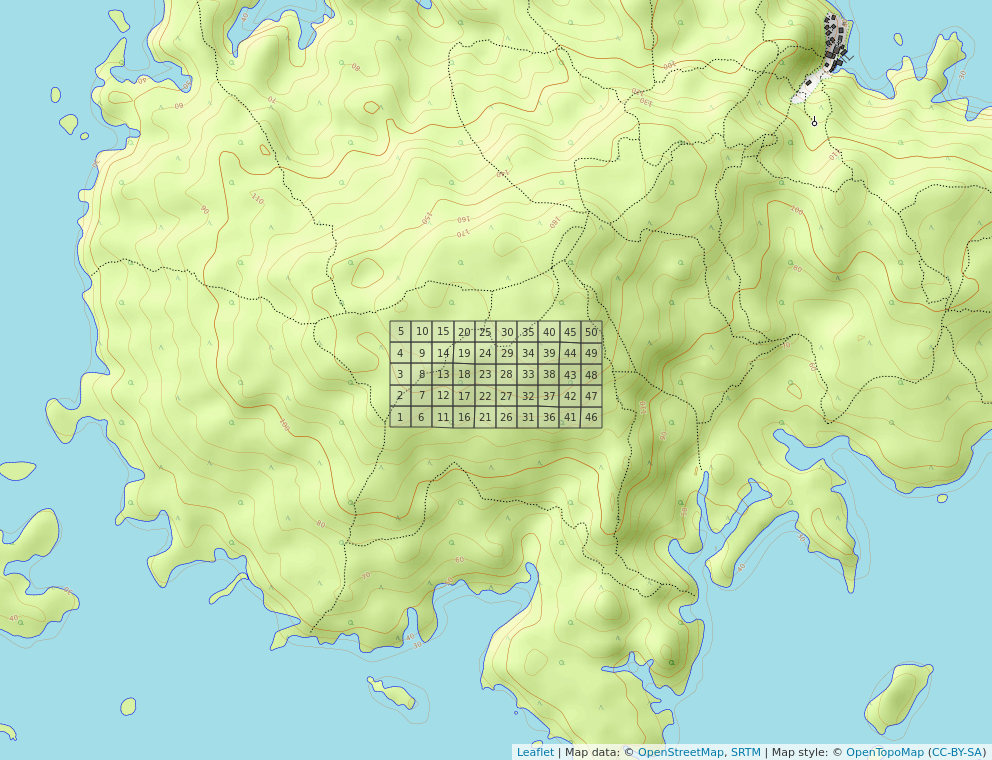
\includegraphics[width=1.00000\textwidth]{mapa_cuadros.png}
\caption{mapa de isla Barro Colorado cuadros\label{fig:bci_map}}
\end{figure}

\begin{figure}
\centering
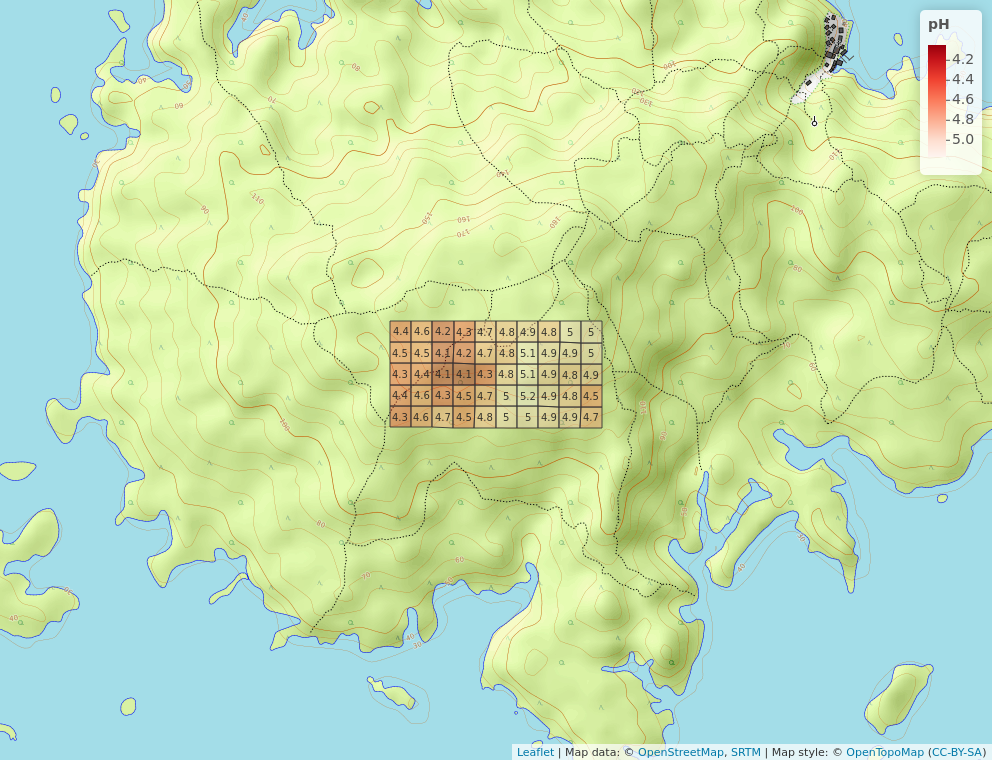
\includegraphics[width=1.00000\textwidth]{mapa_cuadros_ph.png}
\caption{mapa de la isla Barro Colorado cuadros ph\label{fig:bci_map}}
\end{figure}

\begin{figure}
\centering
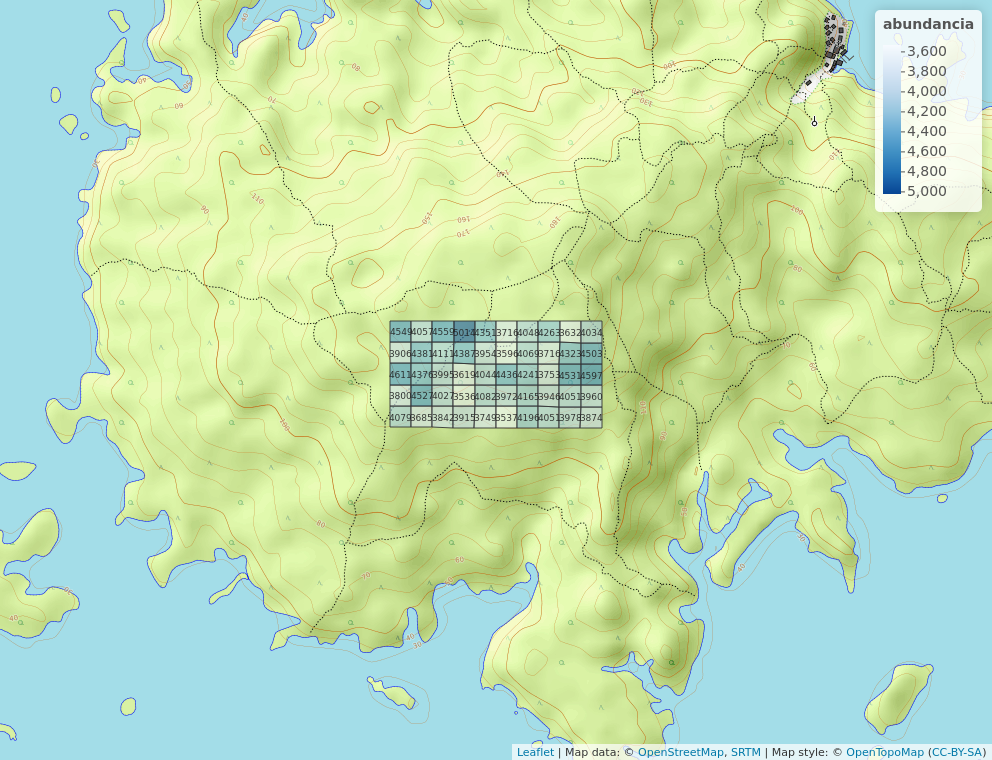
\includegraphics[width=1.00000\textwidth]{mapa_cuadros_abun_global.png}
\caption{mapa de la isla Barro Colorado abundancia global
\label{fig:bci_map}}
\end{figure}

\begin{figure}
\centering
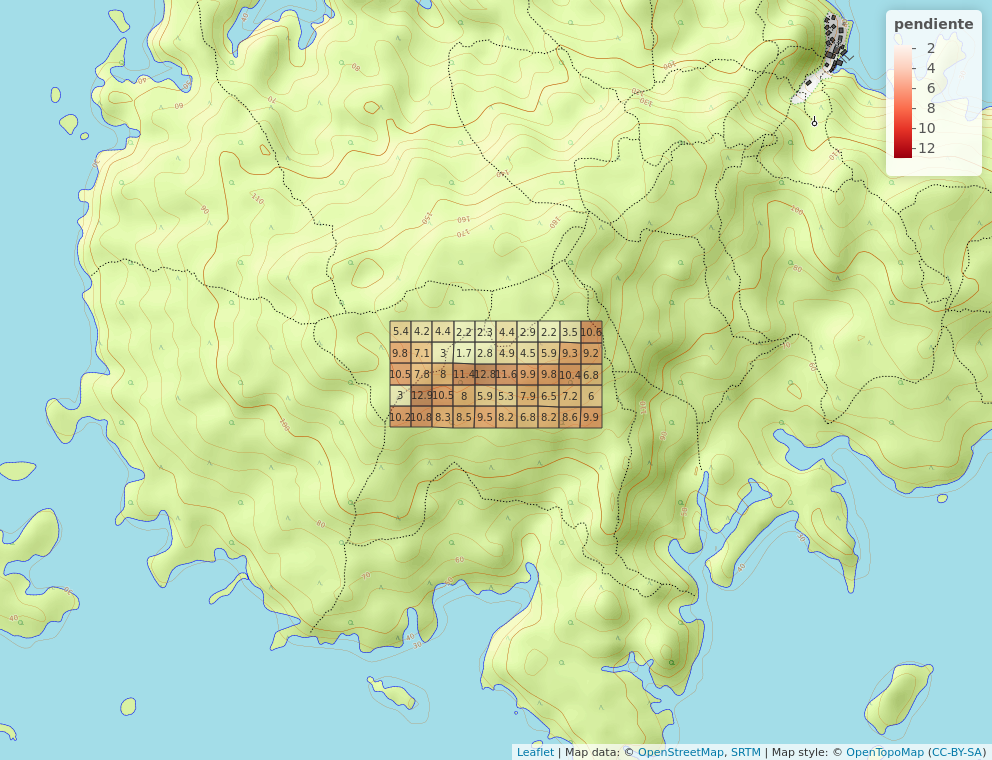
\includegraphics[width=1.00000\textwidth]{mapa_cuadros_pendiente.png}
\caption{mapa de la isla Barro Colorado cuadros y pendientes
\label{fig:bci_map}}
\end{figure}

\begin{figure}
\centering
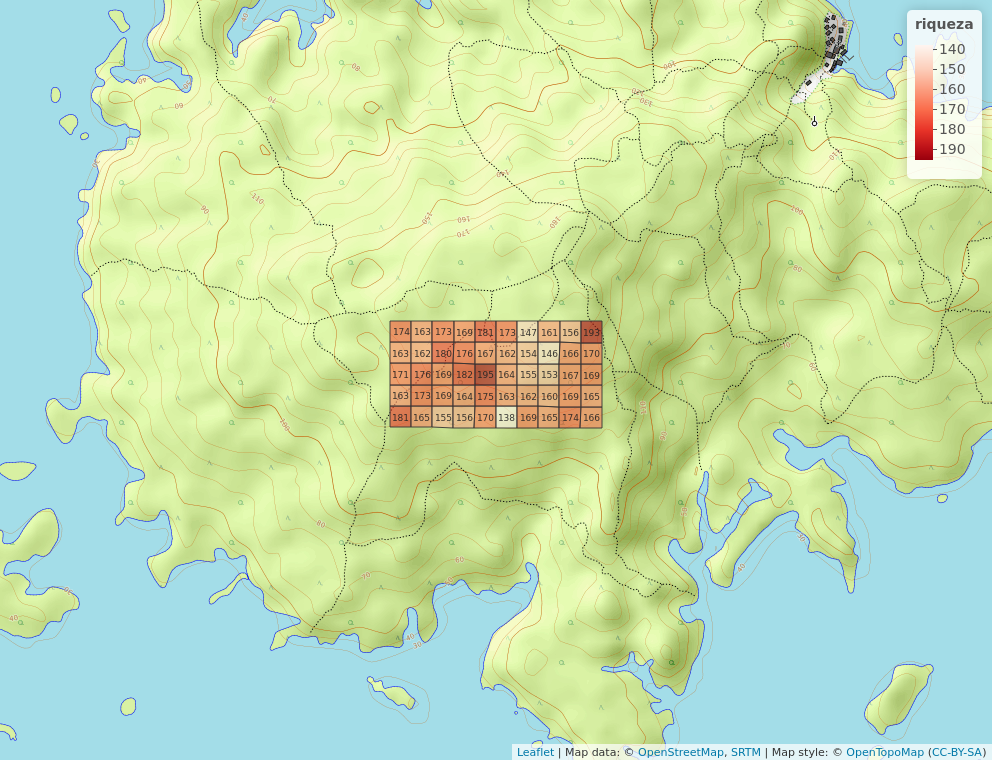
\includegraphics[width=1.00000\textwidth]{mapa_cuadros_riq_global.png}
\caption{mapa de la isla Barro Colorado riquza global
\label{fig:bci_map}}
\end{figure}

\begin{figure}
\centering
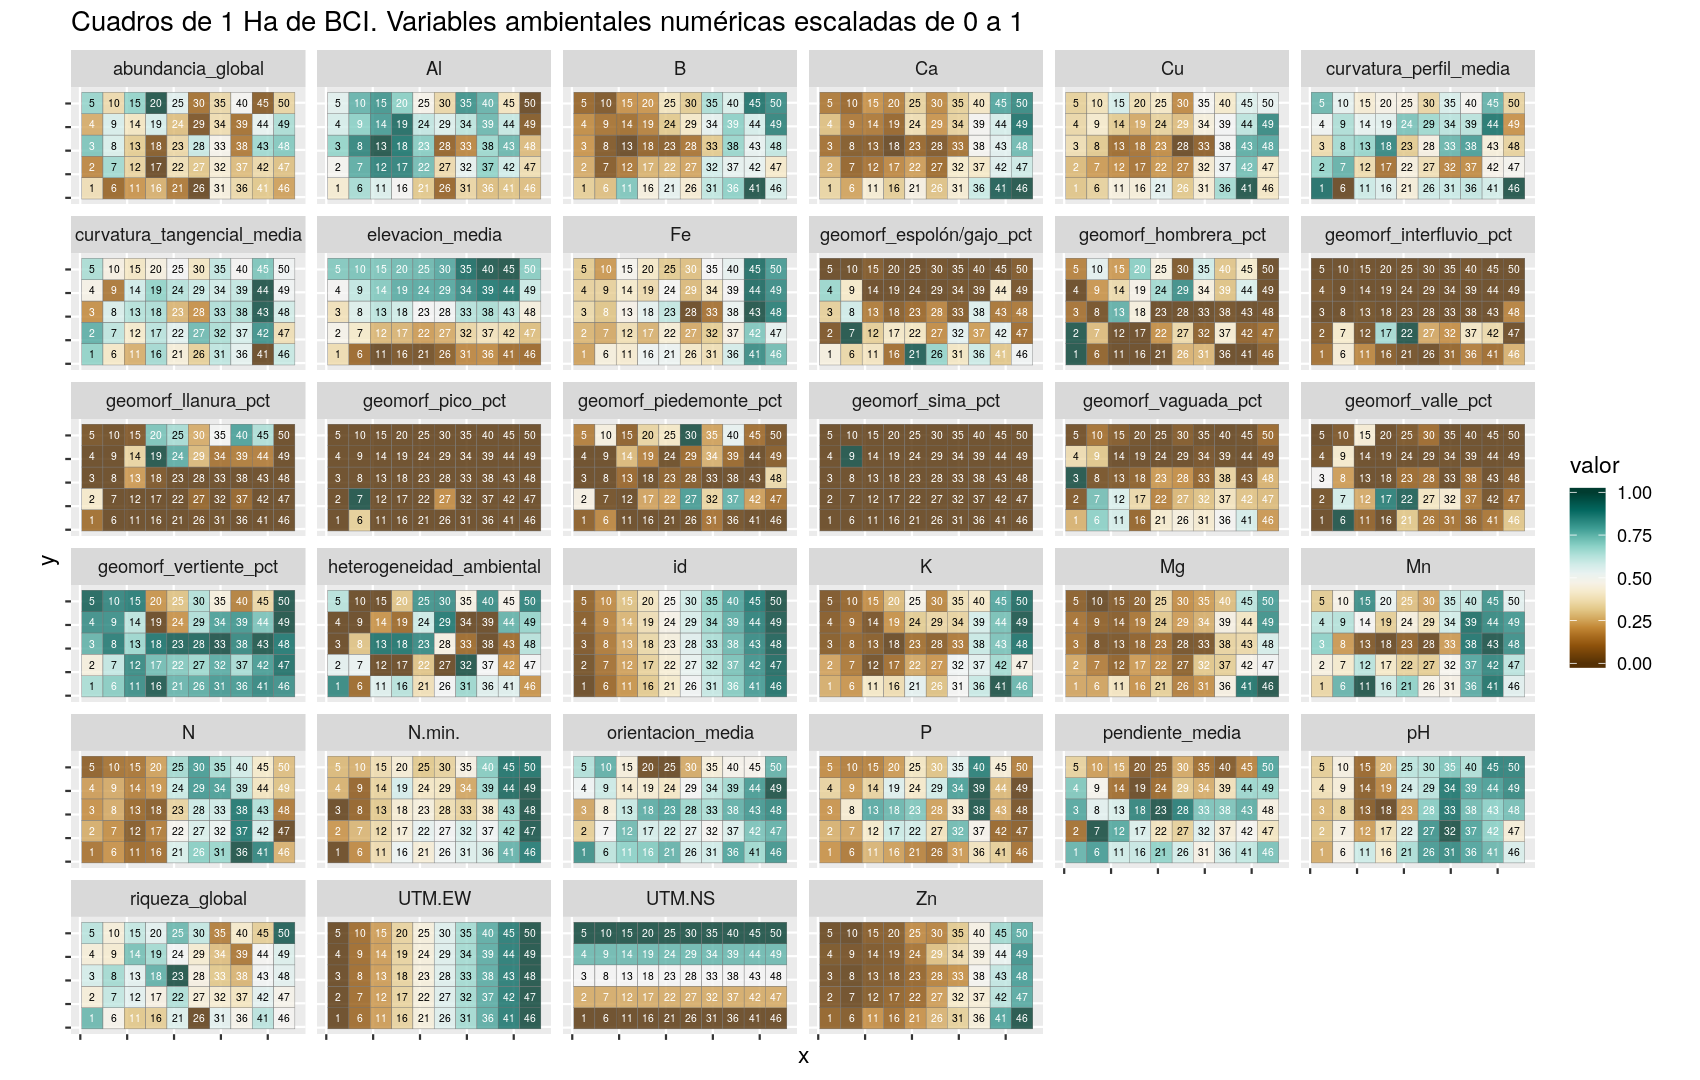
\includegraphics[width=1.00000\textwidth]{mapas_variables_ambientales_numericas.png}
\caption{mapa de la isla Barro Colorado variables ambientales numéricas
\label{fig:bci_map}}
\end{figure}

\begin{figure}
\centering
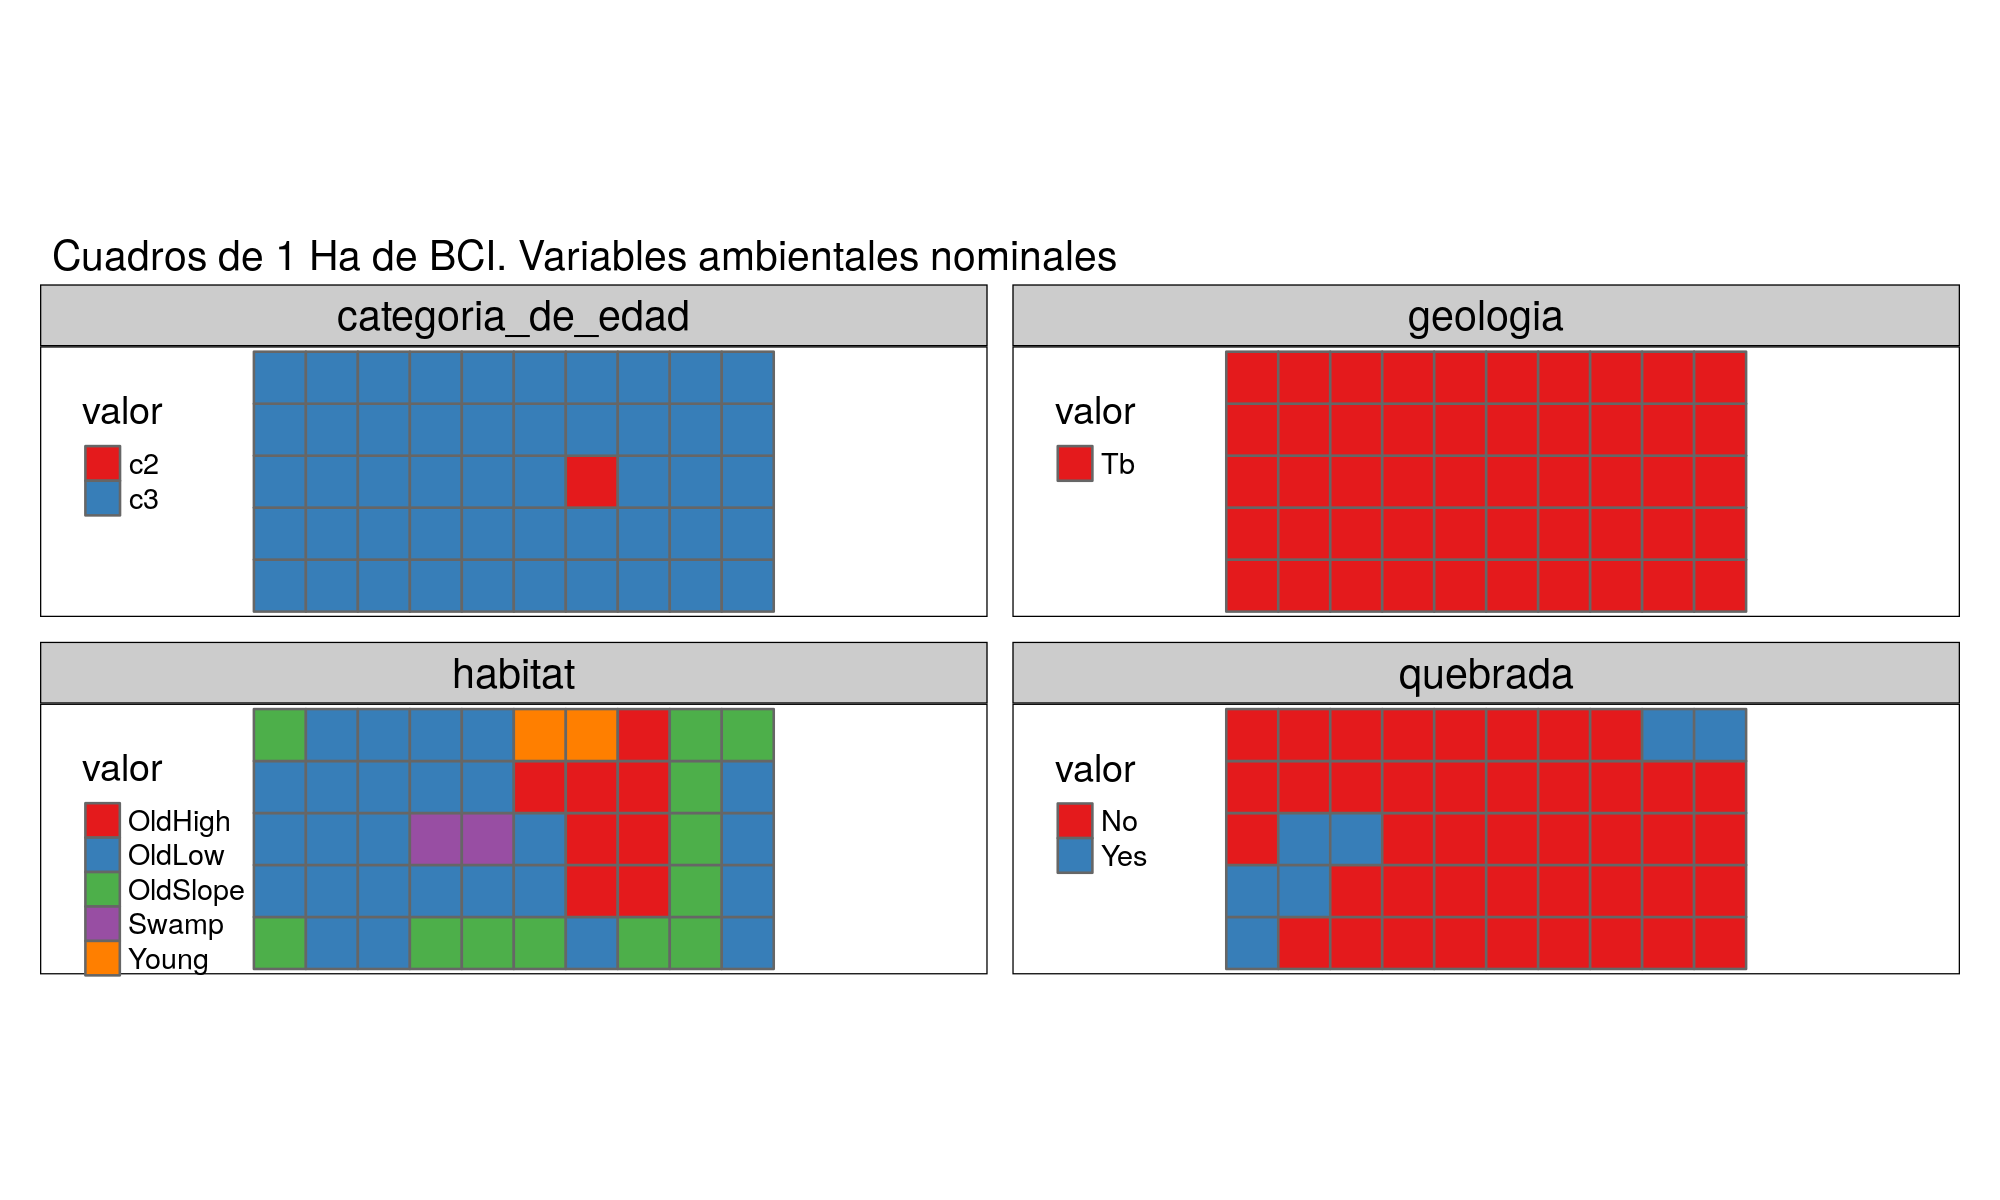
\includegraphics[width=1.00000\textwidth]{mapas_variables_ambientales_nominales_tmap.png}
\caption{mapa de la isla Barro Colorado variables ambientales nominales
\label{fig:bci_map}}
\end{figure}

\begin{figure}
\centering
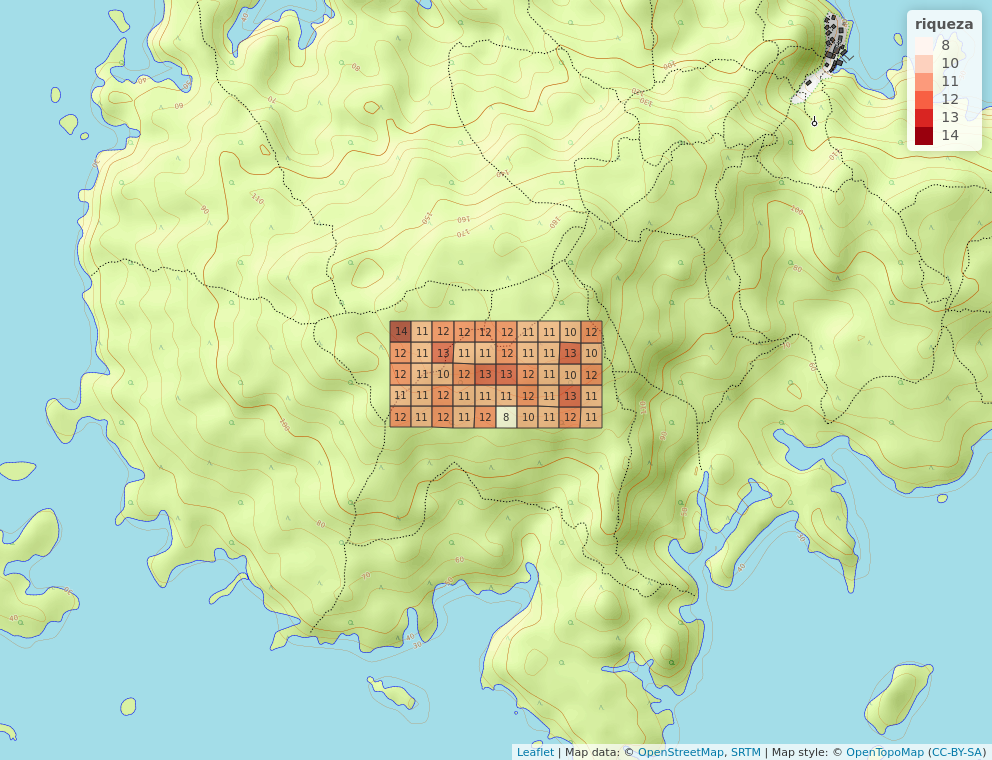
\includegraphics[width=1.00000\textwidth]{mapa_cuadros_riq_mi_familia.png}
\caption{mapa de la isla Barro Colorado cuadro de riqueza mi familia
\label{fig:bci_map}}
\end{figure}

\begin{figure}
\centering
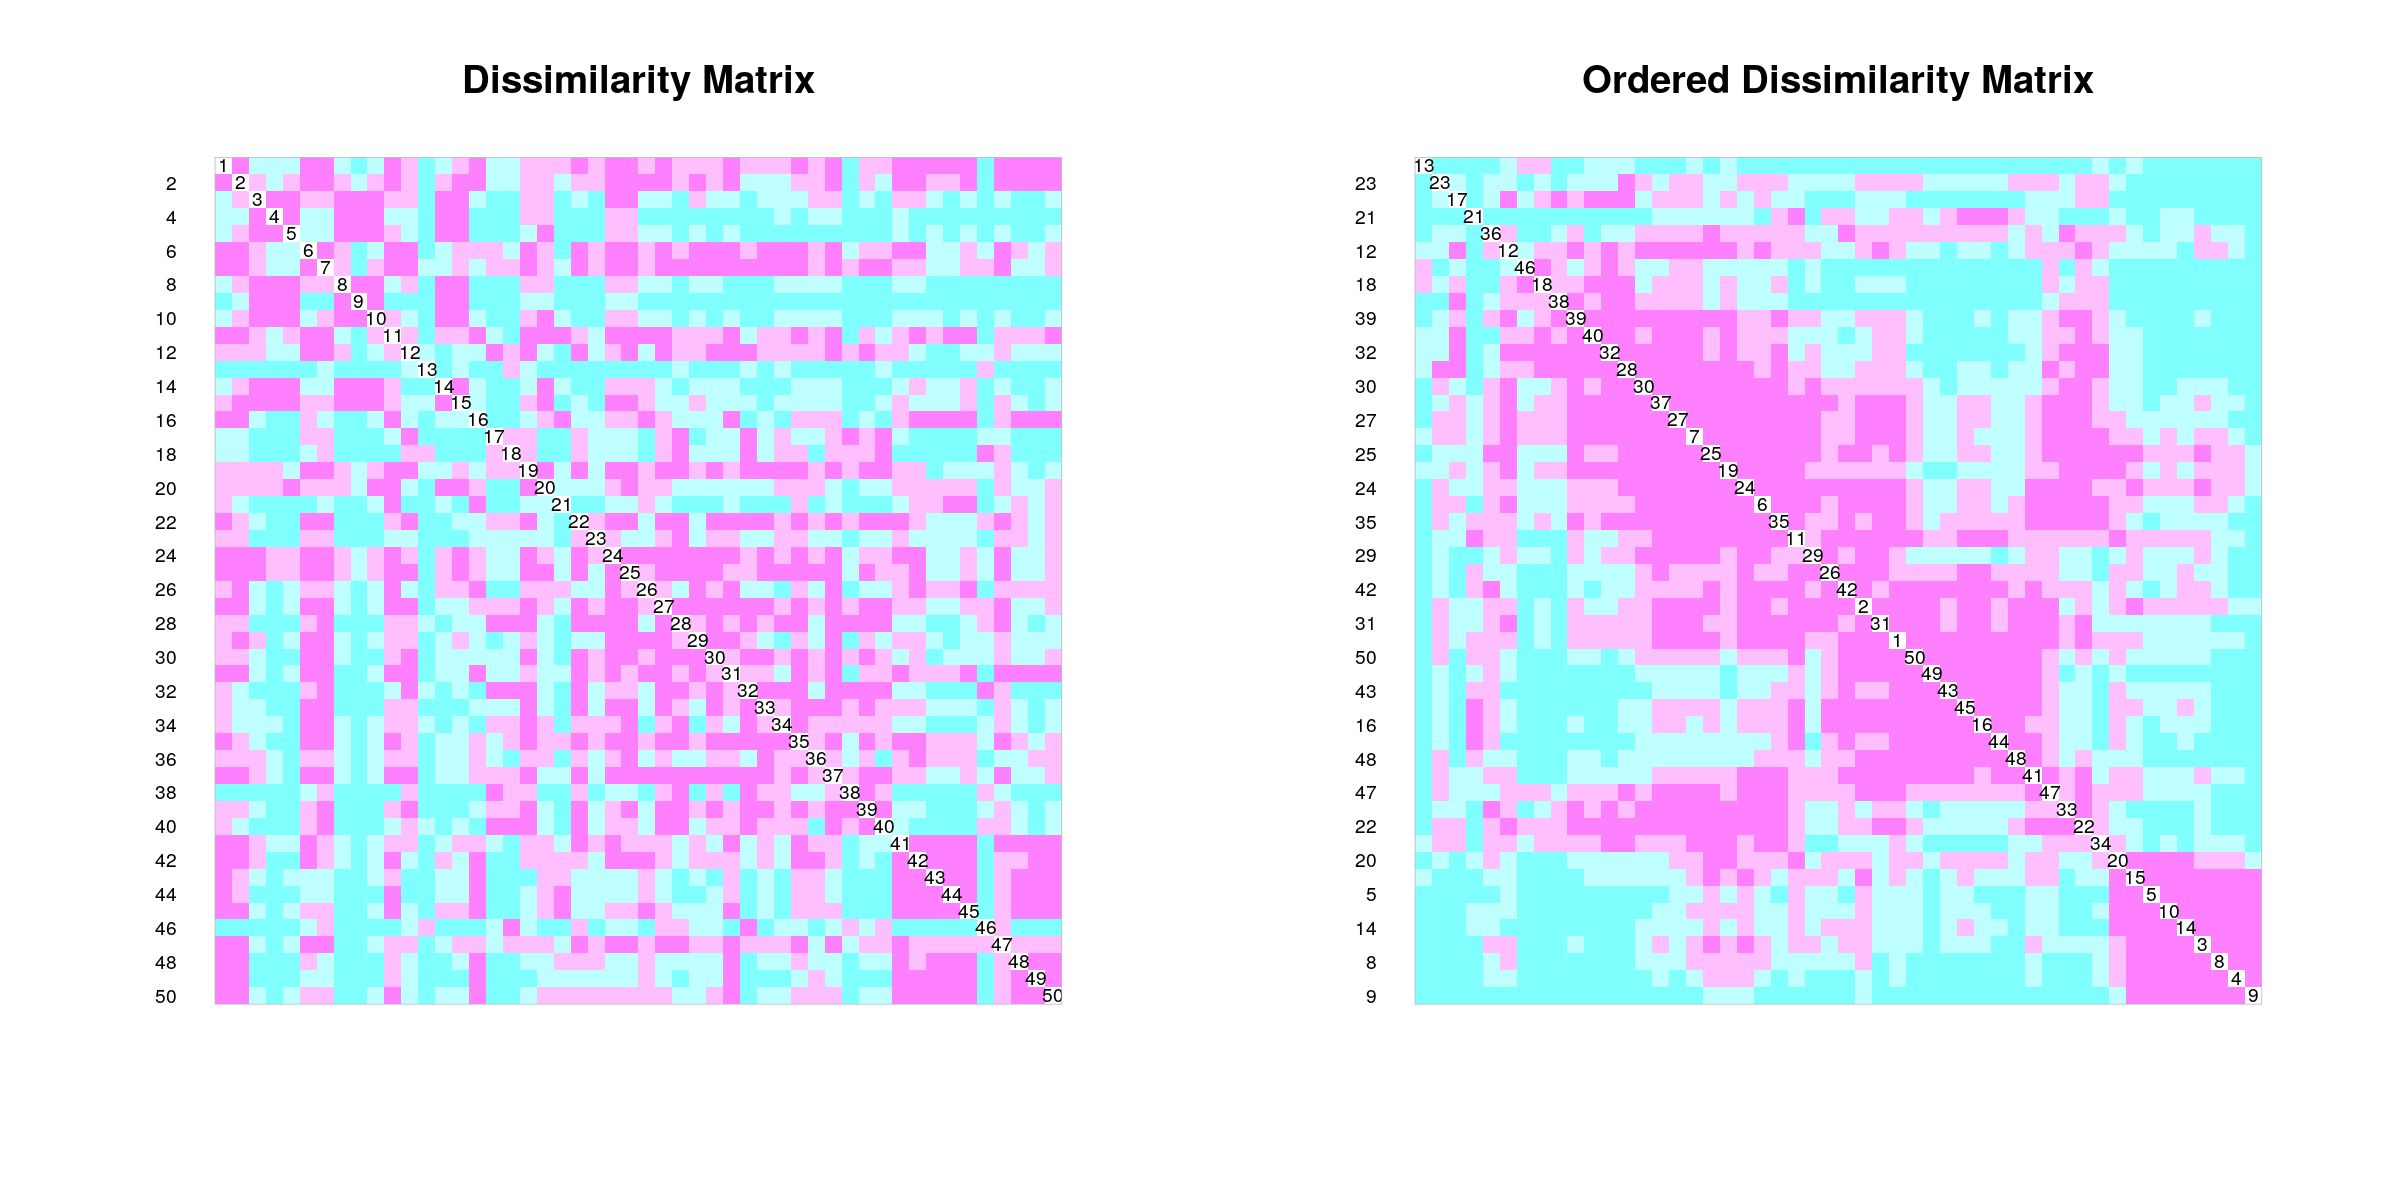
\includegraphics[width=1.00000\textwidth]{matriz_disimilaridad_hellinger.png}
\caption{mapa de la isla Barro Colorado matriz disimilaridad hellinger
\label{fig:bci_map}}
\end{figure}

\begin{figure}
\centering
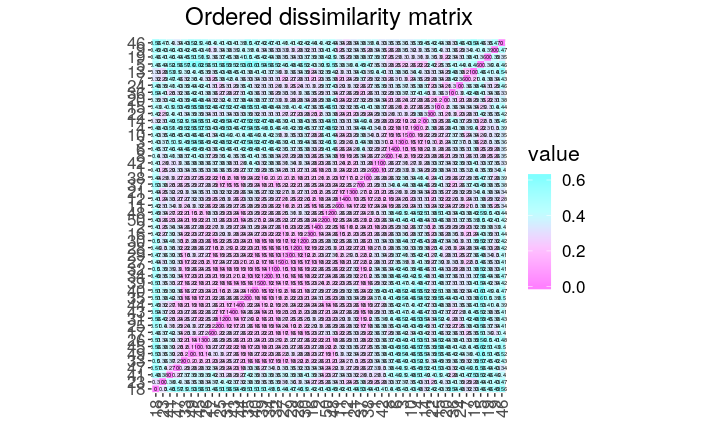
\includegraphics[width=1.00000\textwidth]{matrizdedisimilaridad.png}
\caption{mapa de la isla Barro Colorado matriz disimilaridad
\label{fig:bci_map}}
\end{figure}

\begin{figure}
\centering
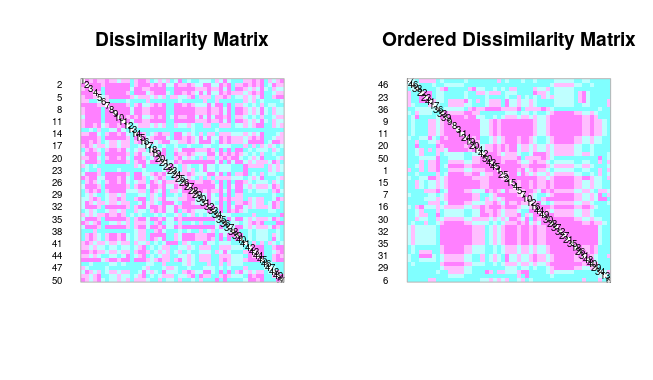
\includegraphics[width=1.00000\textwidth]{matriz_similaridad.png}
\caption{mapa de la isla Barro Colorado matriz disimilaridad
\label{fig:bci_map}}
\end{figure}

\begin{figure}
\centering
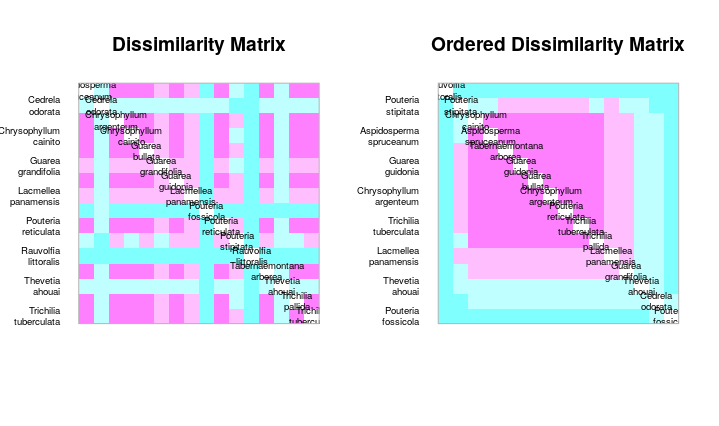
\includegraphics[width=1.00000\textwidth]{mapadecalor.png}
\caption{mapa de la isla Barro Colorado mapa de calor
\label{fig:bci_map}}
\end{figure}

\begin{figure}
\centering
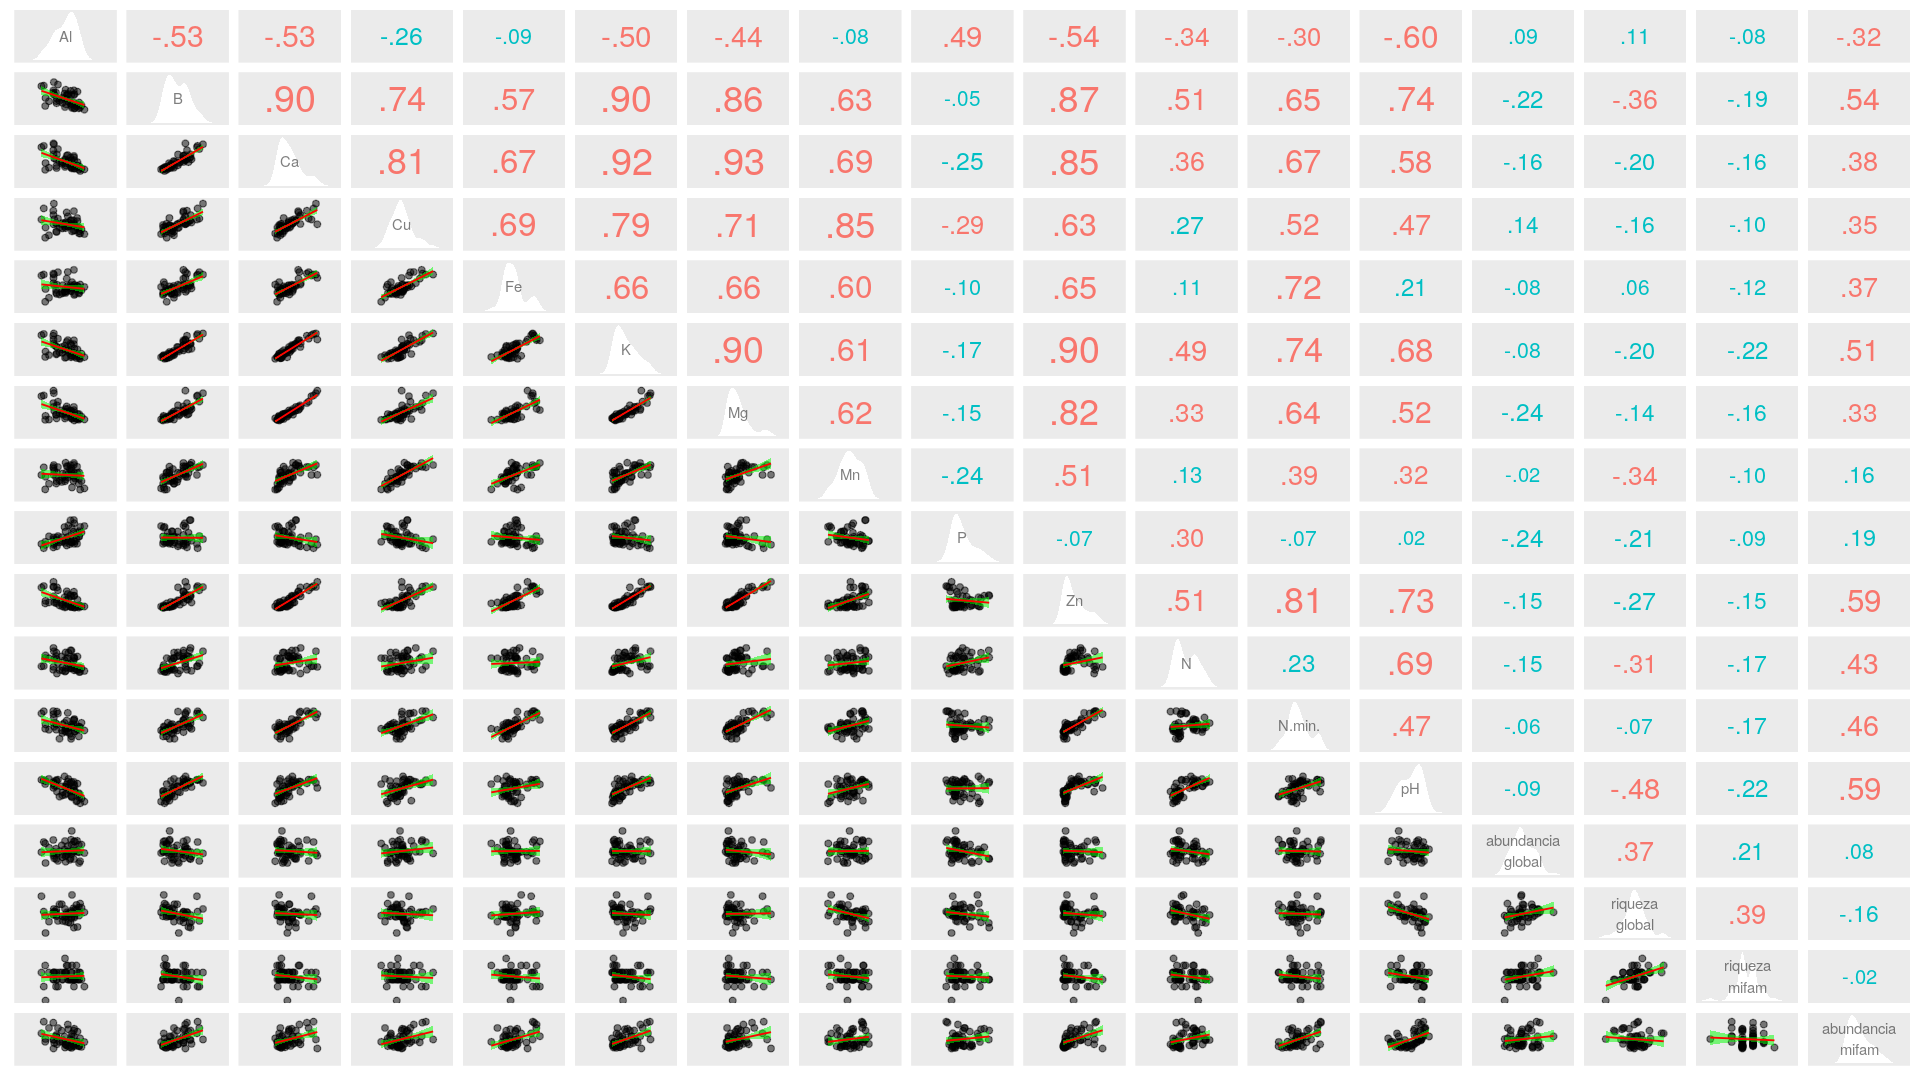
\includegraphics[width=1.00000\textwidth]{matriz_correlacion_suelo_abun_riq_spearman.png}
\caption{mapa de la isla Barro Colorado abundancia y riqueza de suelo
\label{fig:bci_map}}
\end{figure}

\begin{figure}
\centering
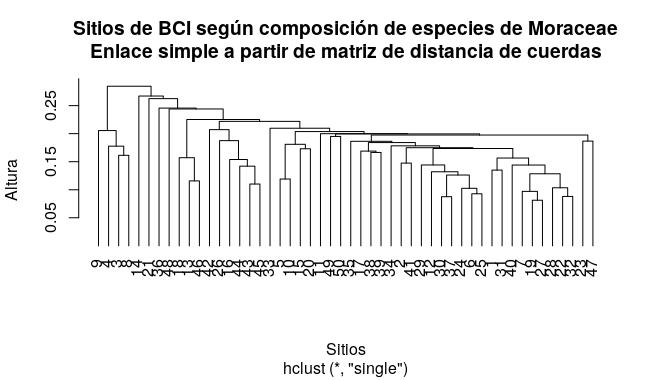
\includegraphics[width=1.00000\textwidth]{sitios_composicion_distancia_cuerdas.png}
\caption{mapa de la isla Barro Colorado sitios de composición por
distancia de cuerda \label{fig:bci_map}}
\end{figure}

\begin{figure}
\centering
\includegraphics[width=1.00000\textwidth]{analisis_interpretacion_dendrogramas.png}
\caption{mapa de la isla Barro Colorado analisis interpretación
dendrogramas \label{fig:bci_map}}
\end{figure}

\begin{figure}
\centering
\includegraphics[width=1.00000\textwidth]{sitios_metodo_ward.png}
\caption{mapa de la isla Barro Colorado sitios de composición por
distancia de cuerda \label{fig:bci_map}}
\end{figure}

\begin{figure}
\centering
\includegraphics[width=1.00000\textwidth]{agrupamiento_dendrograma.png}
\caption{mapa de la isla Barro Colorado sitios de composición por
distancia de cuerda \label{fig:bci_map}}
\end{figure}

\begin{figure}
\centering
\includegraphics[width=1.00000\textwidth]{comparacion_dendrograma_mapa_calor.png}
\caption{mapa de la isla Barro Colorado sitios de composición por
distancia de cuerda \label{fig:bci_map}}
\end{figure}

\begin{figure}
\centering
\includegraphics[width=1.00000\textwidth]{multiescalar_bootstrap.png}
\caption{mapa de la isla Barro Colorado remuestreo multiescalar por
Bootstrap \label{fig:bci_map}}
\end{figure}

\begin{figure}
\centering
\includegraphics[width=1.00000\textwidth]{agrupamiento_dendrogramas_porcentajes.png}
\caption{mapa de la isla Barro Colorado dendrogramas y porcentajes
\label{fig:bci_map}}
\end{figure}

\begin{figure}
\centering
\includegraphics[width=1.00000\textwidth]{mapa_upgma_k2.png}
\caption{mapa de la isla Barro Colorado sitios de composición por
distancia de cuerda \label{fig:bci_map}}
\end{figure}

\begin{figure}
\centering
\includegraphics[width=1.00000\textwidth]{mapas_variables_ambientales.png}
\caption{mapa de la isla Barro Colorado mapa de variables ambientales
\label{fig:bci_map}}
\end{figure}

\begin{figure}
\centering
\includegraphics[width=1.00000\textwidth]{mapa_ward_k3.png}
\caption{mapa de la isla Barro Colorado grupos Ward k3
\label{fig:bci_map}}
\end{figure}

\begin{figure}
\centering
\includegraphics[width=1.00000\textwidth]{cuadro_cajas_ward.png}
\caption{mapa de la isla Barro cuadro de cajas Ward \label{fig:bci_map}}
\end{figure}

\begin{figure}
\centering
\includegraphics[width=1.00000\textwidth]{modelo_abundancia_especie.png}
\caption{mapa de la isla Barro Colorado modelo abundancia de especies
\label{fig:bci_map}}
\end{figure}

\begin{figure}
\centering
\includegraphics[width=1.00000\textwidth]{Numero_individuos.png}
\caption{mapa de la isla Barro Colorado número de individuos
\label{fig:bci_map}}
\end{figure}

\begin{figure}
\centering
\includegraphics[width=1.00000\textwidth]{diversidad_beta.png}
\caption{mapa de la isla Barro Colorado mapa de calor
\label{fig:bci_map}}
\end{figure}

\begin{figure}
\centering
\includegraphics[width=1.00000\textwidth]{mi_fam_hel_pca.png}
\caption{mapa de la isla Barro Colorado diagrama de componentes
principales variables\label{fig:bci_map}}
\end{figure}

\begin{figure}
\centering
\includegraphics[width=1.00000\textwidth]{escalamiento_1_2.png}
\caption{mapa de la isla Barro Colorado diagrama de escalamiento 1 y 2
\label{fig:bci_map}}
\end{figure}

\begin{figure}
\centering
\includegraphics[width=1.00000\textwidth]{rda_escala_especies.png}
\caption{mapa de la isla Barro Colorado RDA diagrama de especies
variables\label{fig:bci_map}}
\end{figure}

\begin{figure}
\centering
\includegraphics[width=1.00000\textwidth]{rda_escalamiento_escala_5.png}
\caption{mapa de la isla Barro Colorado RDA especies no raras
variables\label{fig:bci_map}}
\end{figure}

\begin{figure}
\centering
\includegraphics[width=1.00000\textwidth]{rda_especies_escala_4.png}
\caption{mapa de la isla Barro Colorado RDA digrama de especies
variables\label{fig:bci_map}}
\end{figure}

\includegraphics[width=1.00000\textwidth]{multiples_especies.png} \#
\emph{Script} reproducible

\ldots

\section*{Referencias}\label{referencias}
\addcontentsline{toc}{section}{Referencias}

\hypertarget{refs}{}
\hypertarget{ref-cardona2007avispas}{}
Cardona, W., De Ulloa, P. C., \& Kattan, G. (2007). Avispas no
polinizadoras asociadas a ficus andicola (moraceae) en la cordillera
central de colombia. \emph{Revista Colombiana de Entomología},
\emph{33}(2), 165--170.

\hypertarget{ref-clement2009morphological}{}
Clement, W. L., \& Weiblen, G. D. (2009). Morphological evolution in the
mulberry family (moraceae). \emph{Systematic Botany}, \emph{34}(3),
530--552.

\hypertarget{ref-fredericksenbibosi}{}
Fredericksen, T. S., Justiniano, M. J., Rumiz, D., McDonald, E., \&
Aguape, R. (n.d.). \emph{Bibosi higuerón ficus spp. moraceae}.

\hypertarget{ref-magallanes1972distribucion}{}
Magallanes, A. B., Rocha, Y. R., \& Terán, F. A. (n.d.).
\emph{Distribución y abundancia de las especies arbóreas de la familia
moraceae en la reserva ecológica del mineral de nuestra señora de la
candelaria, cosalá, sinaloa}.

\hypertarget{ref-piedra2006genero}{}
Piedra-Malagón, E. M., Ramírez Rodríguez, R., \& Ibarra -Manríquez, G.
(2006). El género ficus (moraceae) en el estado de morelos, méxico.
\emph{Acta Botánica Mexicana}, (75), 45--75.

\hypertarget{ref-simmonds2002parametros}{}
Simmonds, J. A., Gómez, J. A., \& Villalaz, J. (2002). Parametros
fisico-quimicos y biologicos en aguas circundantes al canal de panama.
\emph{Tecnociencia}, \emph{4}(1), 47--69.

\hypertarget{ref-van2010biodiversidad}{}
Van Devender, T. R., Felger, R. S., Fishbein, M., Molina-Freaner, F. E.,
Sánchez-Escalante, J. J., Reina-Guerrero, A., \& others. (2010).
Biodiversidad de las plantas vasculares. \emph{Diversidad Biológica de
Sonora. Universidad Nacional Autónoma de México. México, DF, México},
229--261.

\hypertarget{ref-williams2002patrones}{}
Williams-Linera, G., \& Meave, J. (2002). Patrones fenológicos.
\emph{Ecología Y Conservación de Bosques Neotropicales, RM Guariguata Y
GH Kattan (Eds .). Libro Universitario Regional, San José}, 591--624.




\newpage
\singlespacing 
\end{document}
